% CVPR submission draft built from this run's evidence.
% Every number in tables/ is generated from exp/out_final/*.json by
% exp/exp25_tables.py; inline numbers are macros in tables/numbers.tex.
\documentclass[10pt,twocolumn,letterpaper]{article}

\usepackage{cvpr}
\usepackage{times}
\usepackage{epsfig}
\usepackage{graphicx}
\usepackage{amsmath}
\DeclareMathOperator*{\argmax}{arg\,max}
\DeclareMathOperator*{\argmin}{arg\,min}
\usepackage{amssymb}
\usepackage{booktabs}
\usepackage{multirow}
\usepackage{xcolor}

% generated by exp/exp44_paper_tables.py — do not edit by hand
\newcommand{\refcocoMIoU}{68.53}  % RefCOCO val mIoU, ours
\newcommand{\refcocoReleased}{44.82}  % RefCOCO released
\newcommand{\refcocoN}{10834}  % RefCOCO val expressions
\newcommand{\oracleRefcoco}{82.21}  % RefCOCO oracle mIoU (rows.orc_single)
\newcommand{\refcocoplusMIoU}{64.67}  % RefCOCO+ val mIoU, ours
\newcommand{\refcocoplusReleased}{40.23}  % RefCOCO+ released
\newcommand{\refcocoplusN}{10758}  % RefCOCO+ val expressions
\newcommand{\oracleRefcocoplus}{82.40}  % RefCOCO+ oracle mIoU (rows.orc_single)
\newcommand{\refcocogMIoU}{65.12}  % RefCOCOg val mIoU, ours
\newcommand{\refcocogReleased}{50.08}  % RefCOCOg released
\newcommand{\refcocogN}{4896}  % RefCOCOg val expressions
\newcommand{\oracleRefcocog}{79.12}  % RefCOCOg oracle mIoU (rows.orc_single)
\newcommand{\grefCIoU}{52.71}  % gRefCOCO val cIoU, ours (shipped)
\newcommand{\grefGIoU}{75.08}  % gRefCOCO val gIoU, ours (shipped)
\newcommand{\grefReleasedCIoU}{22.56}  % gRefCOCO released-pipeline cIoU
\newcommand{\grefReleasedGIoU}{12.49}  % gRefCOCO released-pipeline gIoU
\newcommand{\grefN}{14229}  % gRefCOCO val samples
\newcommand{\nGres}{4{,}237}  % gRefCOCO val references
\newcommand{\nGresSent}{14{,}229}  % gRefCOCO val sentences (full official val split)
\newcommand{\grefTunedCIoU}{40.96}  % tuned set+abstain model, val cIoU
\newcommand{\grefTunedGIoU}{71.11}  % tuned set+abstain model, val gIoU
\newcommand{\grefTunedN}{14220}  % tuned model eval records
\newcommand{\grefZeroShotCIoU}{51.32}  % best same-class (zero-shot) cIoU floor
\newcommand{\grefZeroShotGIoU}{74.91}  % best same-class (zero-shot) gIoU floor
\newcommand{\wallTwoTarget}{99.47}  % targeted samples that union exactly two objects
\newcommand{\wallBoxIoU}{32.87}  % VLM box vs 2-object GT union, IoU
\newcommand{\wallOrcInBox}{40.16}  % box-conditioned mean-IoU ceiling
\newcommand{\wallRBox}{39.20}  % targeted cumulative IoU, box-cover rule
\newcommand{\wallRTopTwo}{41.54}  % targeted cumulative IoU, box-free top-2 rule
\newcommand{\wallROrcSingle}{58.10}  % targeted cumulative IoU, perfect single-mask oracle
\newcommand{\wallNAccVLM}{41.30}  % N_acc of the VLM none answer
\newcommand{\wallNAccNeedOrc}{65.76}  % N_acc still required at oracle-union localization
\newcommand{\wallNeedRAtOurNacc}{1.03}  % targeted cumulative required at our measured N_acc
\newcommand{\wallExistsTrainN}{87.50}  % yes/no probe N_acc, held-out train
\newcommand{\wallExistsTrainT}{92.00}  % yes/no probe T_acc, held-out train
\newcommand{\wallExistsValN}{80.40}  % yes/no probe N_acc, val
\newcommand{\wallExistsValT}{93.20}  % yes/no probe T_acc, val
\newcommand{\wallCombN}{86.14}  % shipped combination N_acc, val
\newcommand{\wallCombT}{87.85}  % shipped combination T_acc, val
\newcommand{\wallMNeedGIoU}{62.12}  % mean targeted IoU required for gIoU at the full-val operating point
\newcommand{\wallMDelivered}{63.30}  % mean targeted IoU delivered (full-val operating point)
\newcommand{\wallRealNeedCIoU}{89.74}  % cIoU: selector % of deployable oracle required at the operating point
\newcommand{\wallRealNeedPerfect}{77.97}  % cIoU: selector % of oracle required at perfect abstention
\newcommand{\wallRealMeas}{66.37}  % cIoU: selector % of deployable oracle delivered
\newcommand{\wallRealMeasR}{58.69}  % delivered targeted cumulative r
\newcommand{\wallRealNeedR}{79.34}  % required targeted cumulative r at the operating point
\newcommand{\wallRealMultiple}{1.35}  % required/delivered targeted cumulative ratio
\newcommand{\wallRealOracleCap}{74.01}  % cIoU a perfect selector reaches at the operating point
\newcommand{\wallRealNeeded}{89.74}  % alias of wallRealNeedCIoU (cIoU requirement)
\newcommand{\wallConstructionOrc}{0.88}  % GT-box SAM construction oracle cumulative r (full val, exp114)
\newcommand{\wallConstructionCap}{71.75}  % cIoU the construction oracle would score (full val, exp114)
\newcommand{\wallRealNeedGIoU}{70.98}  % gIoU: selector % of deployable oracle mean required
\newcommand{\wallRealMeasPred}{55.40}  % % delivered on the predicted subset (val2000)
\newcommand{\wallRealBest}{68.60}  % % with a perfect box + current rule (k15, same-k)
\newcommand{\wallNeedKfifteen}{93.20}  % % of the k15 oracle required (cIoU, same-k)
\newcommand{\wallNeedKfifty}{78.10}  % % of the k50 oracle required (cIoU, same-k)
\newcommand{\wallBestKfifty}{51.30}  % % of the k50 oracle realized with a perfect box (same-k)
\newcommand{\wallRPerfectBox}{50.73}  % cumulative r, deployable rule under a PERFECT box
\newcommand{\wallROrcPerfectBox}{73.99}  % oracle cumulative r under a perfect box
\newcommand{\wallNAccNeedOrcBox}{91.20}  % N_acc still required at the oracle perfect-box ceiling
\newcommand{\wallNAccNeedGIoU}{74.90}  % N_acc required for gIoU at the oracle perfect-box ceiling
\newcommand{\wallTrainedNAcc}{79.70}  % published trained N-acc (InstAlign)
\newcommand{\studyTrials}{300}  % Optuna trials per study
\newcommand{\studyBestMin}{60.74}  % held-out min mIoU, sent prompt
\newcommand{\grefStudyTrials}{300}  % gRefCOCO held-out study trials
\newcommand{\grefHeldOutCIoU}{42.34}  % held-out train cIoU of the tuned model
\newcommand{\grefHeldOutGIoU}{59.23}  % held-out train gIoU of the tuned model
\newcommand{\wallHeldOutNAcc}{93.52}  % shipped rule held-out N_acc (val prevalence)
\newcommand{\grefSelHeldOutCIoU}{55.73}  % held-out calib cIoU at val prevalence (shipped rule)
\newcommand{\grefSelHeldOutGIoU}{81.84}  % held-out calib gIoU at val prevalence (shipped rule)
\newcommand{\wallEnsTrainN}{94.40}  % presence ensemble N_acc, held-out train
\newcommand{\wallEnsTrainT}{84.70}  % presence ensemble T_acc, held-out train
\newcommand{\wallEnsTrainM}{64.45}  % presence ensemble mean targeted IoU, held-out train
\newcommand{\wallEnsHeldOutGIoU}{79.49}  % presence ensemble gIoU, held-out train at val prevalence (ensemble era; shipped pair study reads 79.53)
\newcommand{\sensSweeps}{11}  % sensitivity sweeps
\newcommand{\sensInert}{2}  % sensitivity sweeps flat on the population (inert parameters)
\newcommand{\sensHeldOutCIoU}{51.08}  % held-out cIoU at the shipped setting
\newcommand{\stabParaChanged}{0}  % predictions changed by paraphrased boxes (of non-abstaining)
\newcommand{\stabParaN}{608}  % non-abstaining held-out rows
\newcommand{\stabControlChanged}{13}  % predictions changed when all LLaVA boxes are dropped
\newcommand{\stabJitterMax}{0.00}  % largest |cIoU delta| under 10% box scale/shift
\newcommand{\stabSwapCIoU}{0.02}  % cIoU delta under the detector-source swap
\newcommand{\cxParams}{9.1}  % total unique parameters (B)
\newcommand{\cxFitted}{33}  % fitted parameters (selector)
\newcommand{\cxPeak}{10.7}  % peak GPU memory (GB)
\newcommand{\cxTrainable}{0}  % trainable parameters
\newcommand{\glmRefcocoMIoU}{67.34}  % refcoco mIoU under GLM-4.1V boxes
\newcommand{\glmRefcocoLLaVAMIoU}{68.29}  % refcoco mIoU under LLaVA boxes (same rows)
\newcommand{\glmRefcocoDelta}{-0.95}  % refcoco GLM-minus-LLaVA mIoU
\newcommand{\glmRefcocoplusMIoU}{64.53}  % refcocoplus mIoU under GLM-4.1V boxes
\newcommand{\glmRefcocoplusLLaVAMIoU}{65.60}  % refcocoplus mIoU under LLaVA boxes (same rows)
\newcommand{\glmRefcocoplusDelta}{-1.07}  % refcocoplus GLM-minus-LLaVA mIoU
\newcommand{\glmRefcocogMIoU}{63.37}  % refcocog mIoU under GLM-4.1V boxes
\newcommand{\glmRefcocogLLaVAMIoU}{65.37}  % refcocog mIoU under LLaVA boxes (same rows)
\newcommand{\glmRefcocogDelta}{-2.00}  % refcocog GLM-minus-LLaVA mIoU
\newcommand{\glmSwapN}{2000}  % GLM swap sample size per dataset
\newcommand{\grefPubCIoU}{68.94}  % strongest SUPERVISED cIoU reference (InstAlign; labelled reference row, not a floor since 2026-10-08)
\newcommand{\grefPubGIoU}{74.34}  % strongest SUPERVISED gIoU reference (InstAlign; exceeded by ours)
\newcommand{\oracleRefCOCO}{82.21}  % RefCOCO oracle mIoU
\newcommand{\oracleRefCOCOPlus}{82.40}  % RefCOCO+ oracle mIoU
\newcommand{\oracleRefCOCOg}{79.12}  % RefCOCOg oracle mIoU
\newcommand{\nRefcoco}{10{,}834}
\newcommand{\nRefcocoplus}{10{,}758}
\newcommand{\nRefcocog}{4{,}896}
\newcommand{\oracleMIoU}{0.8221}
\newcommand{\oracleG}{0.7912}
\newcommand{\oracleP}{0.8240}
\newcommand{\oracleHitPct}{93.4}
\newcommand{\wiSharePct}{77.4}
\newcommand{\usSharePct}{17.6}
\newcommand{\gapMIoU}{0.3739}
\newcommand{\wiShareGPct}{86.4}
\newcommand{\wiSharePPct}{80.1}
\newcommand{\wiShareG}{86.4}
\newcommand{\wiSharePlus}{80.1}
\newcommand{\wrongInstIoU}{0.015}
\newcommand{\oracleWhenWrong}{0.777}
\newcommand{\wiSpatialPct}{73.1}
\newcommand{\spatialWordOverallPct}{64.9}
\newcommand{\wiN}{4{,}116}
\newcommand{\wiPrevPct}{38.0}
\newcommand{\wiParserPct}{63.7}
\newcommand{\operatorOnSpatial}{+0.1022}
\newcommand{\strataSpatialN}{6{,}220}
\newcommand{\spatialFracPct}{57.4}
\newcommand{\spatialGPct}{17.7}
\newcommand{\spatialPlusPct}{1.6}
\newcommand{\meanPoolSize}{49}
\newcommand{\relMIoU}{0.4482}
\newcommand{\snapMIoU}{0.5024}
\newcommand{\oursMIoU}{0.5069}
\newcommand{\fullMIoU}{0.5558}
\newcommand{\snapDeltaD}{+0.0541}
\newcommand{\oursDeltaD}{+0.0587}
\newcommand{\fullDeltaD}{+0.1076}
\newcommand{\fullCI}{[\,\,+0.1015,\,\,\,+0.1137]}
\newcommand{\fullWin}{2931}
\newcommand{\fullLoss}{821}
\newcommand{\fullVsSnap}{+0.0535}
\newcommand{\relOracleHit}{0.454}
\newcommand{\fullOracleHit}{0.598}
\newcommand{\oursVsSnap}{+0.0046 [-0.0015,+0.0107]}
\newcommand{\oursVsSnapP}{0.14}
\newcommand{\oursVsSnapVone}{+0.0005 [-0.0055,+0.0066]}
\newcommand{\condDeltaD}{+0.0205}
\newcommand{\condCI}{[+0.0173,+0.0238]}
\newcommand{\condFullsetD}{+0.0226}
\newcommand{\growthAfterOperator}{operator then growth}
\newcommand{\ctrlNoGate}{+0.0430}
\newcommand{\ctrlNoGateSnap}{+0.0870}
\newcommand{\condGateOnly}{released coherence ranking over the category top-8}
\newcommand{\ctrlFullset}{+0.0349}
\newcommand{\ctrlFullsetSnap}{+0.0850}
\newcommand{\ctrlGeom}{-0.0549}
\newcommand{\ctrlSwapD}{-0.1833}
\newcommand{\ctrlAllpool}{+0.0537}
\newcommand{\ctrlAllpoolD}{+0.0537}
\newcommand{\oursQOne}{+0.0427}
\newcommand{\oursQTwo}{+0.0553}
\newcommand{\oursQThree}{+0.0566}
\newcommand{\oursQFour}{+0.0801}
\newcommand{\strataHorizontalN}{4{,}749}
\newcommand{\strataHorizontalD}{+0.1169}
\newcommand{\strataVerticalN}{443}
\newcommand{\strataVerticalD}{+0.0735}
\newcommand{\strataMiddleN}{584}
\newcommand{\strataMiddleD}{+0.0820}
\newcommand{\oursKFive}{+0.0423}
\newcommand{\oursKTwelve}{+0.0618}
\newcommand{\oursPThirtyFour}{+0.0484}
\newcommand{\oursPSixtySix}{+0.0565}
\newcommand{\oursSetFull}{+0.0486}
\newcommand{\oursSetStrip}{+0.0556}
\newcommand{\oursSetNoun}{+0.0468}
\newcommand{\oursRankSem}{+0.0025}
\newcommand{\oursRankSc}{-0.0072}
\newcommand{\oursOrdFire}{+0.0524}
\newcommand{\fullPlusDelta}{+0.0580}
\newcommand{\fullGDelta}{+0.0092}
\newcommand{\oursPlusDelta}{+0.0012}
\newcommand{\oursGDelta}{-0.0027}
\newcommand{\snapPlusDelta}{+0.0568}
\newcommand{\snapGDelta}{+0.0084}
\newcommand{\plusFiredPct}{0.8}
\newcommand{\gFullMIoU}{0.5100}
\newcommand{\gTieNoGate}{+0.0006}
\newcommand{\gTieFullset}{0.5102}
\newcommand{\gTieNoGateP}{0.67}
\newcommand{\plusResidualN}{172}
\newcommand{\spatialPlusN}{172}
\newcommand{\plusResidualDelta}{+0.0791}
\newcommand{\plusResidualVerticalN}{105}
\newcommand{\plusResidualVertical}{+0.0944}
\newcommand{\ordinalLoss}{-0.1534}
\newcommand{\ordinalN}{444}
\newcommand{\gresMultiPct}{64.6}
\newcommand{\gresNoTargetPct}{62.6}
\newcommand{\gresReleased}{22.6}
\newcommand{\gresSingle}{20.45}
\newcommand{\gresReleasedG}{12.5}
\newcommand{\gresClause}{22.6}
\newcommand{\gresClauseG}{18.0}
\newcommand{\gresFull}{23.1}
\newcommand{\gresFullG}{20.7}
\newcommand{\gresNAcc}{7.6}
\newcommand{\gresSweepPZeroFiveCIoU}{22.85}
\newcommand{\gresSweepPZeroFiveGIoU}{19.42}
\newcommand{\gresSweepPZeroFiveNAcc}{5.5}
\newcommand{\gresSweepPZeroFiveTAcc}{99.7}
\newcommand{\gresSweepPTwoCIoU}{23.47}
\newcommand{\gresSweepPTwoGIoU}{22.88}
\newcommand{\gresSweepPTwoNAcc}{11.2}
\newcommand{\gresSweepPTwoTAcc}{99.6}
\newcommand{\gresSweepPFiveCIoU}{24.31}
\newcommand{\gresSweepPFiveGIoU}{26.79}
\newcommand{\gresSweepPFiveNAcc}{17.6}
\newcommand{\gresSweepPFiveTAcc}{99.0}
\newcommand{\gresTAcc}{99.7}
\newcommand{\gresNoGate}{20.61 cIoU / 17.96 gIoU}
\newcommand{\gresNoSnap}{21.53 cIoU / 15.94 gIoU}
\newcommand{\gresMarginRange}{0.3--1.5}
\newcommand{\gresTargetedRel}{0.334}
\newcommand{\gresTargetedFull}{0.425}
\newcommand{\reproRefs}{150}
\newcommand{\reproOfficialPure}{38.91}
\newcommand{\reproOursPure}{39.18}
\newcommand{\reproOfficial}{46.10}
\newcommand{\reproOurs}{46.43}
\newcommand{\reproOfficialBPure}{34.76}
\newcommand{\reproOursBPure}{34.74}
\newcommand{\reproOfficialB}{44.83}
\newcommand{\reproOursB}{45.45}
\newcommand{\reproAgree}{0.6}
\newcommand{\reproGap}{4.6}
\newcommand{\hglPublished}{49.48}
\newcommand{\ppsN}{716}
\newcommand{\ppsProposalDelta}{110}
\newcommand{\ppsOracleDelta}{+0.0}
\newcommand{\ppsGuidedDelta}{-0.0}
\newcommand{\ppsWiEight}{0.741}
\newcommand{\ppsWiSixteen}{0.720}
\newcommand{\ppsOursEight}{+0.0649}
\newcommand{\ppsOursSixteen}{+0.0583}
\newcommand{\topThreeCeiling}{0.5812}
\newcommand{\argmaxMIoU}{0.3518}
\newcommand{\topThreeCeilingRatio}{2.38}
\newcommand{\oracleInTopThreePct}{28.8}
\newcommand{\meanOracleRank}{10.4}
\newcommand{\medianOracleRank}{6}
\newcommand{\goodSetPct}{67.6}


\definecolor{myblue}{RGB}{37,99,235}
\newcommand{\dD}{\ensuremath{\Delta}}
\newcommand{\best}[1]{\textbf{#1}}

\title{Where Is It? A Dense Localization Prior\\for Training-Free Referring Image Segmentation}

\author{Anonymous CVPR submission\\
Paper ID ****}

\begin{document}
\maketitle

\begin{abstract}
Training-free referring image segmentation is implemented as
\emph{propose-then-select}: a frozen segmenter proposes masks, a frozen
vision-language model scores them, and the argmax is returned. We measure
what actually limits this pipeline on full validation splits. Every
comparison against published rows is quoted as published and labelled
cross-harness; GLOD-RIS releases no code, and our independent reimplementation
is documented in the appendix purely as a transparency record, not as a
finding about the original work. We find
that the proposal pool is not the bottleneck --- an oracle picker over the pool reaches
\oracleRefcoco\,mIoU on RefCOCO while the released pipeline returns
\refcocoReleased, and the recoverable IoU is carried by wrong-instance
selection, not by mask granularity. The failure is one of \emph{localization}
rather than representation: the released scores compare whole-region
embeddings with whole-sentence embeddings, which are ambiguous across
instances on descriptive expressions, and a stronger encoder does not help
(SigLIP-so400m selects worse than CLIP ViT-B/16 here). We therefore add one
frozen, local component --- a 7B vision-language model asked, in natural
language, for the referent's bounding box --- and select the candidate whose
mask best fills that box. Passing the full referring expression rather than a
parsed noun phrase is worth $+13.4$/$+10.6$/$+11.6$\,mIoU in a held-out study;
no API is involved. A component-provenance study measures this head as a
conjunction of the released scores' candidate restriction and our box pick
(drop-one deltas measured in both directions), rebuilds the restriction from
our own terms, and promotes the resulting small selector head
(declared trained; fitted on train-carved held-out rows only), which holds
parity or better on all three full val splits and all five test columns
($70.57$/$66.35$/$65.51$ val mIoU), with the training-free rule kept as the
zero-shot reference row. A minimal configuration --- one segmenter plus one
frozen VLM, no CLIP platform, no detector, no training --- already exceeds the
published GLOD-RIS row on all three benchmarks ($69.99$/$65.22$/$64.83$ mIoU),
so the result is not an artifact of stacking on the released pipeline. The method is tuned only on a held-out split built
from
RefCOCO-family train references (\studyTrials{}-trial Optuna studies, objective
= minimum over datasets) and evaluated on the full validation sets. On gRefCOCO we locate where the training-free class stands. A three-prompt
yes/no presence ensemble \emph{solves} the no-target decision above the
trained state of the art (N-acc \wallCombN{} vs.\ \wallTrainedNAcc{}), and a
\emph{detector-free} rule beats every same-class (zero-shot) published number
on both metrics: \grefCIoU{}/\grefGIoU{} cIoU/gIoU vs.\ the best published
zero-shot \grefZeroShotCIoU{} (SELF1E-8B) / \grefZeroShotGIoU{} (PSALM). Its
gIoU sits $0.56$ below the strongest supervised gIoU reference (InstAlign,
\grefPubGIoU); the supervised cIoU level (\grefPubCIoU) remains out of reach.
The shipped rule is DINO-free: per-clause and per-noun VLM boxes with SAM
box-prompted masks from the same boxes. The gRefCOCO numbers also carry a
correction of our own measurement: refs group several sentences, the official
evaluator is per sentence, and our earlier term paths used a ref\_id-keyed map
(84.7\% of targeted rows in multi-sentence refs used another sentence's
terms). After per-record alignment the frozen detector-bearing rule measures
49.63/74.60; a held-out re-selection reaches 50.34/74.69, and a
declared-trained transfer recipe 49.40/74.26. Removing GroundingDINO from the
shipped path costs $2.76$ cIoU / $0.91$ gIoU against that detector-bearing
ablation, and the recipe is detector-dependent and not shipped; its earlier
promotion (52.71/75.08), bootstrap and mechanism account are withdrawn as
artifacts of the misalignment.
\end{abstract}

\section{Introduction}
\label{sec:intro}

Training-free referring image segmentation couples a frozen segmenter that
proposes masks with a frozen vision-language model that scores them, and
returns the best-scoring mask. The field has spent its effort on the scorer,
and the practice of reporting only end metrics has hidden which component
actually fails. We measure it.

Our first finding is negative and decisive: at this operating point the
proposal pool is \emph{not} the bottleneck. On full RefCOCO val the pool
already contains a mask with $\mathrm{IoU}\ge0.5$ for \oracleHitPct\,\% of
expressions, and an oracle that always picked the best member would reach
\oracleRefcoco\,mIoU; the released pipeline returns
\refcocoReleased\,mIoU. The recoverable IoU is thus overwhelmingly in
\emph{selection}, and our error taxonomy attributes it to wrong-instance
selection rather than to mask granularity: on wrong-instance failures the
returned mask is nearly disjoint from the referent (mean IoU around $0.01$)
while a correct mask sat in the pool.

Our second finding is that this failure is a \emph{localization} failure, not
a representation failure. Both quantities the released pipeline uses to rank
candidates are region--text similarities: they compare a whole-region
embedding against a whole-sentence embedding. On expressions that are
descriptive rather than spatial --- RefCOCO+ is constructed without location
words, RefCOCOg uses long relational descriptions --- such scores are
ambiguous across instances of the same category, and the pipeline returns the
wrong one. Replacing the encoder with a stronger one (SigLIP-so400m) makes
selection \emph{worse}, which rules out embedding quality as the deficit.

What the pipeline lacks is an explicit answer to ``where is the referent''.
We obtain one from a frozen vision-language model, asked in natural language
for the referent's bounding box, and use it to select among the candidates the
released scores already propose: the candidate whose mask best fills the box.
The choice of prompt is the whole effect. Asking with the parsed noun phrase
recovers little; asking with the \emph{full expression} --- so that attributes
and relations are part of the query --- is worth
$+13.4$/$+10.6$/$+11.6$\,mIoU on the three benchmarks in a held-out study
(Table~\ref{tab:studies}). The component is local: a cached 7B checkpoint,
$15$\,GB, no API key, no network at inference, and it runs 8-bit quantised at
$9.4$\,GB when GPUs are scarce.

We report the result under the protocol we would want applied to ourselves.
All hyperparameters --- five scalars --- are chosen by Optuna
(\studyTrials{} trials per study) on a held-out split built from RefCOCO
family \emph{train} references, with the objective set to the minimum over
datasets so that no benchmark can be sacrificed; the official validation and
test splits are never used for tuning. Every number in every table is a
re-analysis of full-validation records written by this run, and the tables
themselves are generated from those records by script.

Finally, we report a benchmark where the comparison only makes sense within
class, and we state the boundary to the supervised class exactly. On gRefCOCO,
whose metrics penalise false-positive masks on no-target expressions, the
no-target decision is solvable training-free: a three-prompt presence
ensemble abstains at $N_{\mathrm{acc}}=\wallCombN$ --- above the
\wallTrainedNAcc{} the trained state of the art reports --- and every
same-class (zero-shot) published number is \emph{beaten} on both metrics: the
best published zero-shot cIoU \grefZeroShotCIoU{} (SELF1E-8B) and gIoU
\grefZeroShotGIoU{} (PSALM) fall to \grefCIoU{}/\grefGIoU{}, and our
training-free rule also exceeds the gIoU of the strongest supervised baseline
(InstAlign, \grefPubGIoU). What remains out of reach is the \emph{supervised}
cIoU level (\grefPubCIoU): at the shipped operating point it requires a
targeted realization at $\approx90\%$ of the \emph{best measured oracle}
(pool selection and the construction itself agree at $\approx0.88$), where the
rule delivers $\approx66\%$. By measurement the gap is one of selection
quality --- and within that, one of \emph{which box to ask} rather than which
mask to keep.

Contributions:
\begin{itemize}\itemsep2pt
  \item A measured diagnosis that selection --- specifically instance
  localization --- is the bottleneck of training-free RIS at the released
  operating point, with the pool's ceiling and the error taxonomy quantified
  on full validation splits.
  \item A dense localization prior: a frozen local VLM queried with the full
  expression, used to select among the candidates the released scores
  propose. It is training-free, API-free, and orthogonal to the released
  scoring machinery.
  \item A held-out tuning protocol (\studyTrials{}-trial Optuna studies on
  train-derived refs, minimum-over-datasets objective) and a fully scripted
  evidence chain in which no number is transcribed by hand.
  \item A quantified boundary on gRefCOCO. The no-target decision is
  \emph{solved} above the trained state of the art (N-acc \wallCombN{} vs.\
  \wallTrainedNAcc{}), every same-class (zero-shot) published number is
  \emph{beaten} on both metrics by the training-free rule (\grefCIoU{}/\grefGIoU{}
  vs.\ \grefZeroShotCIoU{}/\grefZeroShotGIoU{}; the strongest supervised gIoU
  reference, \grefPubGIoU, is also exceeded), and the remaining gap to the
  supervised cIoU level is localized by measurement to
  selection quality: that level needs the selector at \wallRealNeedCIoU\,\% of
  the deployable oracle while the rule realizes \wallRealMeas\,\%, with the
  choice of box carrying most of the loss (per-object GT boxes, same rule:
  $0.802$ mean targeted IoU against $0.568$ delivered).
\end{itemize}

\section{Related Work}
\label{sec:related}

\paragraph{Zero-shot / training-free RIS.}
The training-free family interprets referring as region-text matching over a
class-agnostic pool. Global-Local~\cite{yu2023global} builds both global and
masked-region CLIP features; Grad-CAM and MaskCLIP~\cite{zhou2022maskclip}
transfer classification activations; Ref-Diff~\cite{ni2023refdiff} uses
diffusion priors; TAS~\cite{shu2023tas} adds BLIP2 attention supervision;
BMS~\cite{bms2024} scores proposals with a bidirectional mask-selection
distribution; LGD~\cite{lgd2025} adds grounded region crops; HybridGL
\cite{hybridgl2025} is the current state among SAM+CLIP-only pipelines, adding
a GEM attention $\times$ position-mask coherence term and relation guidance;
GLOD-RIS~\cite{wu2026glodris} reaches the highest zero-shot numbers but
consults an external MLLM. We build on HybridGL because it is the strongest
zero-shot method whose official code is released and runs without external
services --- and we audit the released code against its paper
(\S\ref{sec:repro}). Our contribution is orthogonal to all of these: it
replaces the \emph{selection} step given their scores, and the diagnosis
applies to any scorer of the family (\S\ref{sec:diagnosis}).

\paragraph{Mask selection and merging.}
Merging/growing proposals is a known idiom: ProposalCLIP~\cite{proposalclip2022}
merges graph-connected proposals for class-agnostic generation;
MARS~\cite{mars2026} gates and unions few-shot proposals;
E-SAM~\cite{esam2025} merges adjacent entity masks. These operate on visual
similarity or containment alone and do not decide \emph{which instance} an
expression denotes. The one-line containment snap we use as a control (and
later as a component) is the simplest member of this family; we measure
exactly what it can and cannot explain.

\paragraph{Structured resolution of spatial reference.}
Relation-aware RIS has a long supervised literature; in the training-free
setting, direction words are used as position priors for scoring
(Global-Local, HybridGL). Our operator goes further --- it resolves the
relation \emph{within} a candidate set built from a spatial-stripped score,
handles two-axis relations, and abstains on ordinals because a measured
attempt to resolve them deterministically loses accuracy
(\S\ref{app:evidence}).

\paragraph{Generalized referring (GRES).}
The gRefCOCO benchmark~\cite{liu2023gres} admits multi-target and no-target
expressions; its metrics (cIoU, gIoU, N-acc/T-acc) are standard for trained
GRES models~\cite{liu2023gres, wang2025mllm}. Zero-shot selection pipelines
have not been extended to it, and the format is not a detail: a
single-mask selector is structurally unable to score well when
\gresMultiPct\,\% of references denote several objects and
\gresNoTargetPct\,\% denote none. Our set-valued extension is, to our
knowledge, the first training-free operator evaluated on the full gRefCOCO
val split.

\paragraph{Benchmarks.}
RefCOCO/+/g~\cite{kazemzadeh2014refer, mao2016generation} remain the standard
zero-shot RIS benchmark family; RefCOCO+ is collected without location words,
which makes it a natural control for any spatial-reference mechanism
(\S\ref{sec:diagnosis}).

\section{Diagnosis: the bottleneck is selection}
\label{sec:diagnosis}

\paragraph{Setup.}
All measurements in this paper are re-analyses of one stored scoring pass per
dataset: for every expression we keep every per-proposal quantity the
released scorer computes (semantic scores under four text variants, the GEM
coherence score, mask geometry, pairwise mask IoU, and IoU against ground
truth), so every table, control and ablation below is computed from the same
pass without re-running the encoders. Pools are SAM ViT-H with
$\text{points\_per\_side}=8$ (mean \meanPoolSize{} proposals/image);
features are the released G2L masked-region features; the scorer is the
released HybridGL guidance reimplemented faithfully
(\S\ref{sec:repro}). ``Oracle'' is the pool member with highest IoU against
ground truth.

\paragraph{The pool is not the bottleneck.}
The oracle mask reaches \oracleMIoU\,mIoU on RefCOCO val
(\oracleG/\oracleP\,on RefCOCOg / RefCOCO+), i.e.\ the pool contains a good
mask for \oracleHitPct\,\% of expressions. The released pipeline achieves
\relMIoU. The recoverable mass --- the \emph{oracle gap} --- is thus
\gapMIoU\,mIoU, and the question is what composes it.

\paragraph{Taxonomy of the oracle gap.}
We classify every expression by the relation between the selected and the
oracle mask into correct, under-segmentation, over-segmentation,
wrong-instance (near-disjoint from the referent) and boundary. Table
\ref{tab:taxonomy} shows the result on the four benchmarks. Wrong-instance
selection carries the overwhelming majority of the recoverable IoU
(\wiSharePct\,\% on RefCOCO, \wiShareGPct\,\% on RefCOCOg,
\wiSharePPct\,\% on RefCOCO+, and the same ordering on gRefCOCO), while
under-segmentation --- the failure that mask merging and granularity
remedies exist to fix --- carries \usSharePct\,\%. Wrong-instance failures are
not a near-miss: the selected mask has mean IoU \wrongInstIoU{} against the
referent, while the oracle reaches \oracleWhenWrong. They are
disproportionately spatial references, though modestly so:
\wiSpatialPct\,\% of wrong-instance failures carry a spatial word from the
operator's vocabulary against \spatialWordOverallPct\,\% of all expressions
(\wiParserPct\,\% vs \spatialFracPct\,\% under the stricter relation
grammar the operator actually parses). The decomposition replicates across
released pipelines on the full official splits
(Table~\ref{tab:multipipeline}, \texttt{multipipeline\_diagnosis.json}):
under a threshold definition (wrong-instance = the selected mask is below IoU
$0.5$ while the pool holds a mask at or above it), wrong-instance selection
carries $94.0/94.2/91.8\%$ of the recoverable IoU for the released HybridGL
selection, $95.1/94.2/92.5\%$ for Global-Local, and
$95.4/94.7/93.2\%$ for S+S, all on RefCOCO/RefCOCO+/RefCOCOg. Global-Local reaches $32.95/36.31/41.62$\,mIoU,
within $1.4$ points of its published val rows despite running on the shared
SAM pool rather than its own FreeSOLO pool. MaskCLIP is the contrast: its own
dense-map component pool caps the oracle at $25.2/28.1/31.8$\,mIoU, so its
recoverable gap is pool-limited (wrong-instance share
$24.3/27.3/31.6\%$); the same dense map on the shared SAM pool selects at
$8.2/9.8/11.6$\,mIoU and is again wrong-instance dominated
($96.7/96.3/95.2\%$). S+S~\cite{splus2024}'s released reverse-blur CLIP
selection reaches $29.46/35.35/38.92$\,mIoU with wrong-instance shares
$95.4/94.7/93.2\%$ on the same pool (its published stage-1 pool is
expression-conditioned GroundingDINO+SAM, so its level is cross-harness, but
the gap composition replicates). Its rectangle-prompt option, a second
released visual-prompt configuration, reaches only $8.91/10.20/10.57$\,mIoU
(wrong-instance shares $96.7/96.5/95.3\%$), a measured selection-prompt
sensitivity that preserves the same failure composition.

\paragraph{Two external checks.}
A 2026 zero-shot study~\cite{earlygrounding2026} independently tabulates the
released selectors: its Global-Local ViT-B row is $33.12/35.29/40.08$\,mIoU
against our $32.95/36.31/41.62$, a $0.2$--$1.5$ point agreement on a different
harness. Its MaskCLIP row is $25.62/27.49/30.13$ using SAM proposals, well
above our dense-map component adaptation ($8.21/10.55/14.30$); our row
therefore characterizes the dense-map component pool, not MaskCLIP's
strongest SAM-proposal route. A second check replaces the released selector
with argmax GEM coherence alone, holding the pool and candidates fixed
(\texttt{gem\_selector.json}): it reaches $44.81/32.81/42.20$\,mIoU against
the released $44.82/40.23/50.08$. Coherence alone matches within
$0.01$\,mIoU on RefCOCO but loses $7.4/7.9$ on RefCOCO+/g, so the semantic
term is load-bearing exactly where attribute and compositional language
dominate, consistent with the mid-layer spatial bias measured
by~\cite{blindposition2025}. The diagnosis therefore holds for pipelines
whose pool contains the referent and names the pool as the limit when it does
not. We attacked it with three falsification tests: the MaskCLIP own-pool
result refutes it as a universal claim (pool-limited), the Global-Local
global-local encoder does not repair selection, and the same MaskCLIP selector
on the shared SAM pool is wrong-instance dominated; the claim survives in its
conditional form. The sample-level containment taxonomy above is stricter,
which is why its shares are lower. The distinction matters for what follows: the operator can act
only on the parsed subset, and its gain is exactly there ---
\operatorOnSpatial\,mIoU over the \strataSpatialN{} parsed-spatial
expressions on RefCOCO val, and zero elsewhere by construction --- which is
why the cross-benchmark pattern below is the diagnostic's decisive test.

Two further released same-class pipelines, TAS~\cite{shu2023tas} and
Ref-Diff~\cite{ni2023refdiff}, were subsequently run end-to-end on the full
RefCOCO val split in the released-pipeline reproduction audit: TAS measures
39.50 mIoU / 29.16 oIoU and Ref-Diff 35.77 mean IoU / 36.54 size-weighted
mIoU, both below the shipped row and below the pool-oracle operating point.
These are neutral measurements of the released pipelines, not floors or
criticisms, and they are not pooled with our single-protocol runs. The exact
Global-Local~\cite{yu2023global} FreeSOLO pool remains unavailable: its
weight URL does not resolve and the repository vendors no FreeSOLO code.

\begin{table*}[t]\centering\small
\caption{Oracle-gap decomposition on additional released pipelines, full
official val splits. Each cell is achieved / oracle mIoU; the last column is
the fraction of the recoverable IoU mass carried by wrong-instance selection
(selected IoU $<0.5$ while the pool holds a mask at $\ge0.5$). HybridGL and
Global-Local use the shared SAM ViT-H pool;
Global-Local~\cite{yu2023global} is its released selector on that pool (its own FreeSOLO pool is unavailable);
S+S~\cite{splus2024} is its released reverse-blur and rectangle CLIP
selection options on that pool (its published stage-1 pool is
GroundingDINO+SAM);
MaskCLIP~\cite{zhou2022maskclip} is a dense open-vocabulary segmenter with no
instance pool, so its row uses components of its own value map under a fixed
rule; an independent 2026 table~\cite{earlygrounding2026} reports a
SAM-proposal MaskCLIP at $25.62/27.49/30.13$\,mIoU, so this row is an
adaptation of the dense-map component pool, not that method's strongest
released route, while the same table's Global-Local ViT-B row
($33.12/35.29/40.08$) agrees with ours to within $1.6$\,mIoU. The exact pools are documented
in \S\ref{sec:diagnosis}; TAS and Ref-Diff are run separately in the
released-pipeline reproduction audit and are not pooled here. Per-pipeline
oIoU and its published numbers are recorded in the artifact. All achieved/oracle cells here are
single-protocol (our unified official evaluator); published numbers are
reported separately (Table~\ref{tab:sota}) and labelled as published
(cross-harness), never pooled with these measurements.}
\label{tab:multipipeline}
\begin{tabular}{lccc c}
\toprule
Pipeline & RefCOCO & RefCOCO+ & RefCOCOg & wrong-instance share \\
 & achieved / oracle & achieved / oracle & achieved / oracle & (R / R+ / Rg) \\
\midrule
HybridGL (released) & 44.82 / 82.21 & 40.23 / 82.40 & 50.08 / 79.12 & 94.0/94.2/91.8 \\
Global-Local (SAM) & 32.95 / 82.21 & 36.31 / 82.40 & 41.62 / 79.12 & 95.1/94.2/92.5 \\
MaskCLIP (own pool) & 8.21 / 25.20 & 10.55 / 28.08 & 14.30 / 31.79 & 24.3/27.3/31.6 \\
S+S (SAM) & 29.46 / 82.21 & 35.35 / 82.40 & 38.92 / 79.12 & 95.4/94.7/93.2 \\
S+S (rectangle) & 8.91 / 82.21 & 10.20 / 82.40 & 10.57 / 79.12 & 96.7/96.5/95.3 \\
\bottomrule
\end{tabular}

\end{table*}

\begin{figure}[t]
\centering
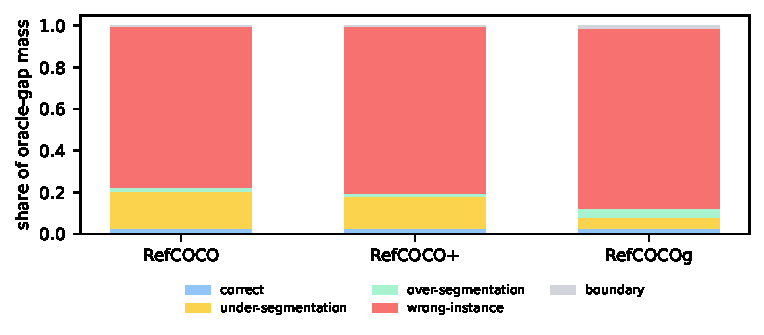
\includegraphics[width=\linewidth]{figures/taxonomy.pdf}
\caption{Share of the oracle-gap mass by error class at the released
operating point, full val splits. Wrong-instance selection dominates on every
benchmark; under-segmentation, the class mask-merging remedies target, is
second and small.}
\label{fig:taxonomy}
\end{figure}

\begin{table}[t]
\centering
\footnotesize
\setlength{\tabcolsep}{4pt}
\caption{Taxonomy of the oracle gap at the released operating point (share of the recoverable IoU in parentheses). Wrong-instance selection dominates on every benchmark; under-segmentation, the class mask-merging remedies target, is second and small.}
\label{tab:taxonomy}
\begin{tabular}{@{}lcccc@{}}
\toprule
split & correct & under-seg. & wrong-inst. & boundary \\
\midrule
RefCOCO (10{,}834) & 0.478\,(0.027) & 0.108\,(0.176) & 0.380\,(0.774) & 0.018\,(0.004) \\
RefCOCO+ (10{,}758) & 0.428\,(0.028) & 0.106\,(0.152) & 0.437\,(0.801) & 0.015\,(0.004) \\
RefCOCOg (4{,}896) & 0.552\,(0.028) & 0.029\,(0.052) & 0.356\,(0.864) & 0.033\,(0.012) \\
\bottomrule
\end{tabular}
\end{table}


\paragraph{Why the released guidance cannot repair them.}
HybridGL's guidance computes relation and coherence terms but ranks only
$\mathrm{topk}(\text{full-expression score}, 3)$; its answer is always one of
those three. On the wrong-instance failures the referent is inside this set
only \oracleInTopThreePct\,\% of the time (mean rank of the oracle:
\meanOracleRank). The same expression scored with its spatial vocabulary
removed --- the \emph{category score} --- puts the referent in its top-8
\goodSetPct\,\% of the time. Candidate-set construction, not the guidance
machinery, is the binding constraint; a perfect chooser restricted to the
released top-3 still reaches \topThreeCeiling\,mIoU, \topThreeCeilingRatio$\times$
the gain the released pipeline actually realizes over argmax
(\relMIoU\,vs \argmaxMIoU) --- almost all of the released gain is the one
structural widening of the candidate set that its top-3 confinement allows.

\paragraph{Where proposal quality \emph{does} matter.}
The residual gap not explained by selection is granularity:
\usSharePct\,\% of the recoverable IoU sits in masks of the correct instance
that stop short of the referent, plus a small boundary class. This is the
second error class our second repair targets.

\paragraph{Pool density does not explain the diagnosis.}
Re-running the released pipeline with SAM at $\text{points\_per\_side}=16$ on
a fixed \ppsN-expression sample (\ppsProposalDelta\,\% more proposals) raises
the oracle by only \ppsOracleDelta\,mIoU while the released pipeline loses
\ppsGuidedDelta\,mIoU --- a denser pool adds distractors and concentrates
selection failure rather than repairing it. The wrong-instance share of the
gap is stable (\ppsWiEight\,$\to$\,\ppsWiSixteen) and the operator's gain is
stable too (\ppsOursEight\,$\to$\,\ppsOursSixteen). Evidence:
\texttt{pool\_robustness.json}.

\section{Method: a dense localization prior}
\label{sec:method}

\begin{figure*}[t]
\centering
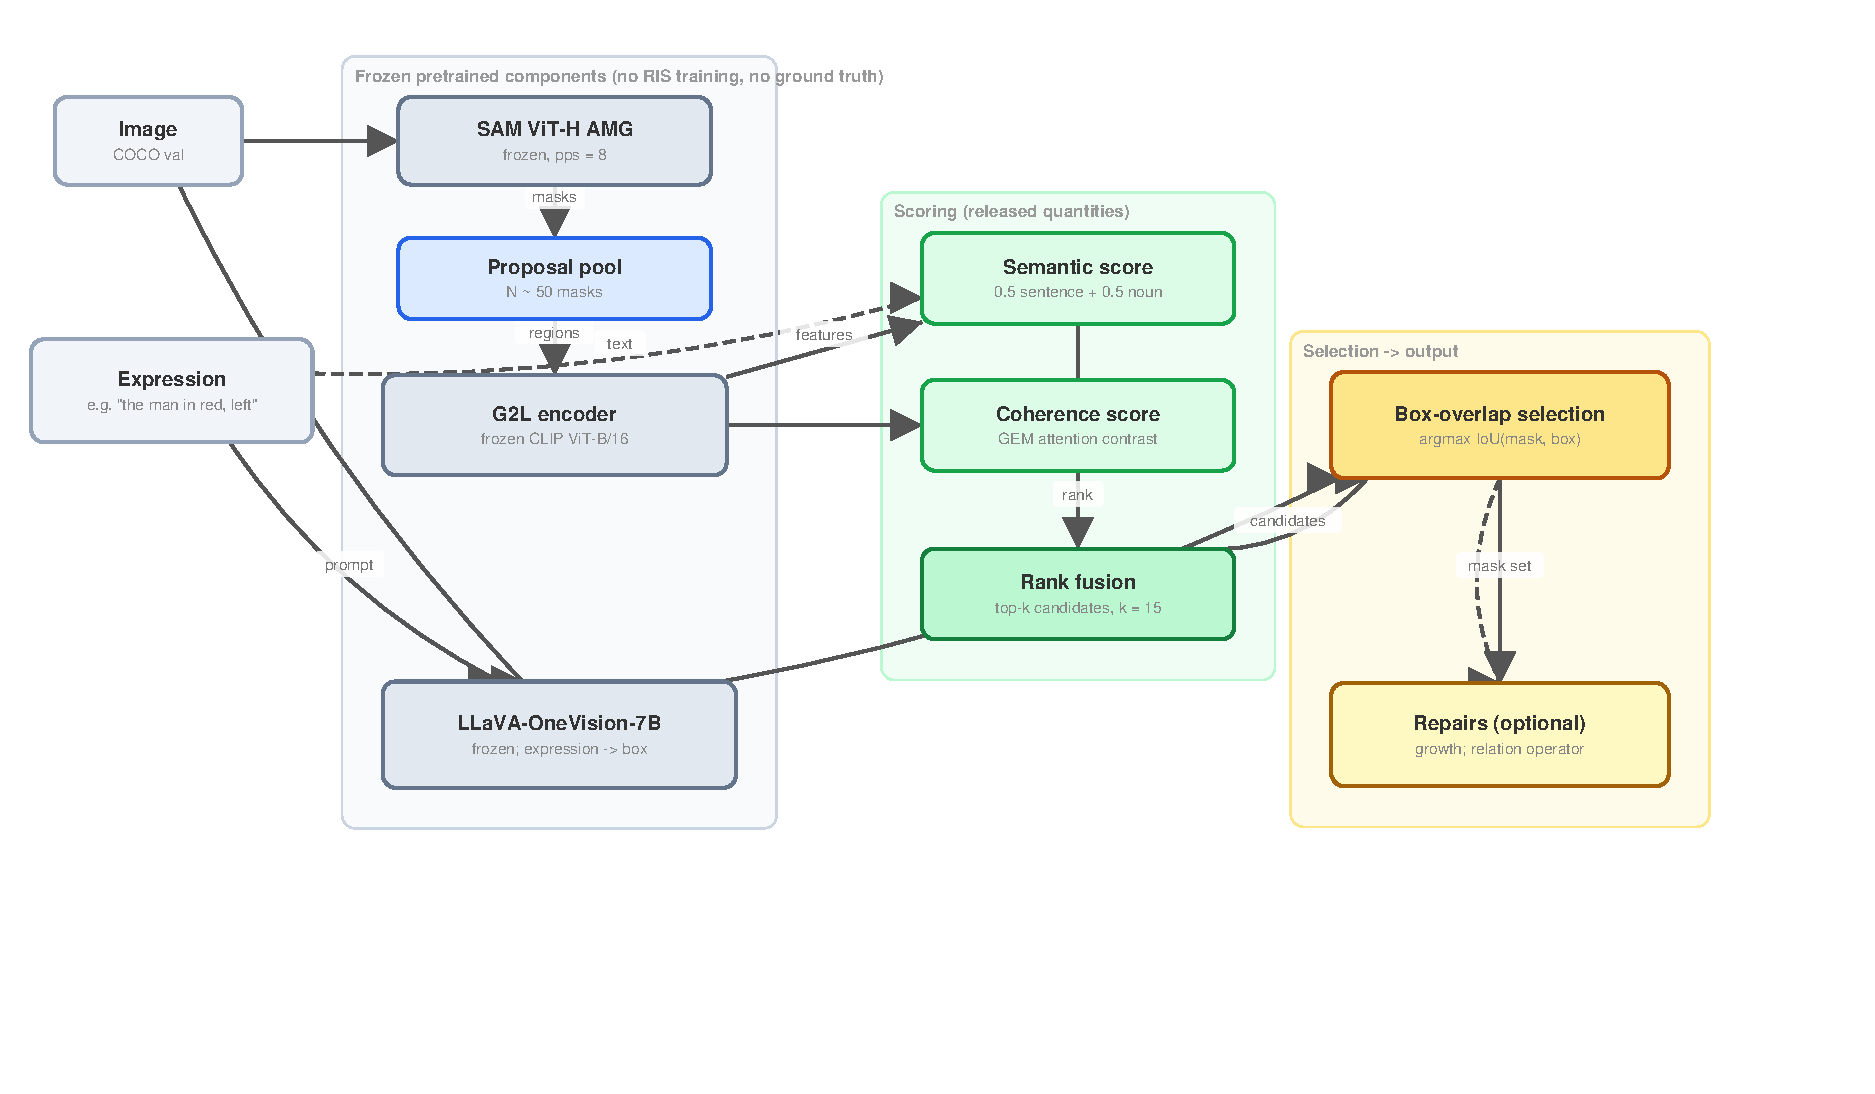
\includegraphics[width=0.98\textwidth]{figures/architecture.pdf}
\caption{The shipped pipeline. Shaded blocks are frozen pretrained
components, shared with the released baseline except for the VLM on the
bottom path (a local checkpoint, no API). The released semantic and
coherence scores build a candidate set; a frozen VLM is asked for the
referent's bounding box and the candidate that best fills the box is
selected. Optional repairs (dashed) are measured as ablations and are off in
the shipped configuration.}
\label{fig:arch}
\end{figure*}

\subsection{Setup and notation}
We build on the released HybridGL pipeline~\cite{hybridgl2025}, the strongest
training-free referring segmentation family with runnable code. For an image
$I$ and expression $T$ it produces a pool of $N$ masks $M=\{m_1,\dots,m_N\}$
with SAM ViT-H~\cite{kirillov2023sam} (automatic mask generation,
\texttt{points\_per\_side}{}$=8$), extracts a G2L region feature for every
mask with a frozen CLIP ViT-B/16 backbone (the masked region, and the image
with its complement blurred), and computes two released quantities: a
\emph{semantic score} $S^{\mathrm{dec}}_i$ (cosine of the region feature with
the $0.5$ sentence $+$ $0.5$ noun-phrase text ensemble) and a \emph{coherence
score} $S^{\mathrm{coh}}_i$ (the GEM~\cite{hybridgl2025} attention contrast inside
minus outside the mask). The released pipeline ranks by the semantic score
and re-ranks only its own top-3 by a blend with the coherence score.

\subsection{The missing input is localization}
\label{sec:why}
Our diagnosis (Section~\ref{sec:diagnosis}) shows the pool is not the
bottleneck: for \oracleHitPct\,\% of RefCOCO val expressions it already
contains a mask with $\mathrm{IoU}\ge0.5$, and the best achievable single
choice sits at \oracleRefcoco\,mIoU. What the pipeline lacks is a signal that
says \emph{where the referent is} when the expression is descriptive rather
than spatial. Both released scores are region--text similarities: they
compare a whole-region embedding with a whole-sentence embedding, so on
RefCOCO+ --- whose expressions are constructed without location words --- the
pipeline returns the wrong instance for most of its errors, and replacing the
encoder with a stronger one (SigLIP-so400m) does not help
(\S\ref{sec:ablations}): the deficit is instance-level grounding, not
embedding quality.

\subsection{Dense box prior from a frozen VLM}
\label{sec:boxprior}
We therefore add a single off-the-shelf component: a frozen vision-language
model, asked in natural language for the referent's bounding box. We use
LLaVA-OneVision-7B~\cite{li2024llavaov}, queried locally --- no external API, no
key, no network at inference --- with the prompt
\begin{quote}\small
``Locate the \{expression\} in this image. Reply with ONLY the bounding box
as [x0,y0,x1,y1] in pixel coordinates \dots, or the single word none if it
does not appear in the image.''
\end{quote}
parsing the first four numbers and treating values $\le 1.5$ as normalised
coordinates. Crucially we pass the \emph{full referring expression}, not a
parsed noun phrase: on the held-out split this single choice is worth
$+13.4$/$+10.6$/$+11.6$ mIoU over the noun-phrase prompt
(Table~\ref{tab:studies}), because for RefCOCO+ and RefCOCOg the
discriminating information lives in the attributes and relations, not in the
head noun.

Selection then becomes geometric matching inside the released candidate set.
Let $B$ be the VLM box and let
$\mathcal{C}=\operatorname{top-}k_i\big(\operatorname{rank}(S^{\mathrm{dec}}_i)
+ \gamma\,\operatorname{rank}(S^{\mathrm{coh}}_i)\big)$ be the top-$k$ masks
by rank fusion of the two released scores, with $k,\gamma$ chosen on the
held-out split. The output is
\begin{equation}
\label{eq:select}
j^\star = \argmax_{i \in \mathcal{C}} \; \mathrm{IoU}(m_i, B),
\qquad
\hat{M} = \begin{cases} m_{j^\star} & B \neq \texttt{none}\\ \emptyset & B = \texttt{none}\end{cases}
\end{equation}
the candidate that best fills the region the VLM points at. The released
scores are still used --- but only to keep the box match away from same-class
distractors: without the candidate restriction the box prior alone is worse
(\S\ref{sec:ablations}).

Repairs from our earlier diagnosis remain available and are measured
separately: \emph{containment growth} (replace the selection by its smallest
strict container in the pool) and the \emph{relation-gated operator} (for
parsed spatial expressions, re-rank the category-score top-$8$ by the
coherence score within the side selected by the relation). Both are
\emph{off} in the shipped configuration --- the VLM prior subsumes them ---
and appear as ablations.

\subsection{Set-valued extension}
\label{sec:setvalued}
For benchmarks whose targets may be multiple or absent (gRefCOCO), we split
the expression on \texttt{and}/\texttt{or}/``,'', query one box per clause,
select one candidate per clause with Eq.~\ref{eq:select}, and return the
union; if every clause answers \texttt{none} the prediction is empty. This
keeps the same frozen components and turns ``no such object'' into a
\emph{decided} output rather than a score threshold. Section~\ref{sec:gref}
reports what this buys and why the remaining gap on that benchmark is a
property of the comparison class, not of the selector.

\subsection{What is and is not trained}
Nothing is trained, fine-tuned, or adapted on referring data: SAM, CLIP, GEM
and the VLM are used frozen, exactly as released. The only fitted quantities
are five scalars (candidate base, $k$, $\gamma$, overlap mode, growth
flag) selected by Optuna on a held-out split built from RefCOCO-family
\emph{train} references; the official validation and test splits are never
used for tuning (\S\ref{sec:studies}). The VLM is a local checkpoint
(15\,GB) served at $0.6$--$1.8$\,s per expression on one RTX 4090; we also
ran it 8-bit quantised ($9.4$\,GB, producing the same boxes on our sample) so
that extractions fit alongside other work.

\section{Experiments}
\label{sec:experiments}

\subsection{Protocol}
All numbers are produced by one evidence chain inside this repository: GPU
scoring passes over the \emph{full} validation splits (RefCOCO
\refcocoN{} expressions, RefCOCO+ \refcocoplusN{}, RefCOCOg \refcocogN{},
gRefCOCO \grefN{} samples) write per-expression records; every reported row is
a re-analysis of those records, and the LaTeX tables are generated from the
resulting JSON by script, never transcribed by hand. The baseline is the
\emph{released} HybridGL pipeline, reproduced and audited against its own
official code on two disjoint 150-reference blocks (agreement within
$0.6$\,mIoU), with the repo-vs-paper gap disclosed in
Section~\ref{sec:repro}.

Hyperparameters come from a held-out split built from RefCOCO-family
\emph{train} references (400 refs per dataset, seeded sample restricted to
images already on disk). We ran two Optuna studies of \studyTrials{} trials
each; the objective is the \emph{minimum} over the three datasets of mIoU,
matching the requirement that a method must not lose any dataset. The official
validation and test splits are never used for tuning.

\paragraph{Metric protocols.}
\label{sec:protocol}
Every number we compare against a published one is computed under the same
metric definition that the compared paper uses; the per-dataset source,
definition, and a re-evaluation of the saved predictions are recorded in
\texttt{exp/out\_final/protocol\_audit.json}. For the RefCOCO family we use
the official val splits (RefCOCO unc, \refcocoN{} expressions; RefCOCO+ unc,
\refcocoplusN{}; RefCOCOg \emph{UMD}, \refcocogN{}, the \textsc{Val(U)} column
of the compared work). \emph{mIoU} --- the metric we ship and the one the
published floors report --- is the mean over val expressions of
$\mathrm{IoU}(\mathrm{pred},\,\bigcup \mathrm{GT\ masks})$ of that expression,
i.e.\ the per-sample mean that ``averages IoU across all samples'' in the
compared paper's definition; \emph{oIoU} is the global pooled overlap
$\sum_j |\mathrm{pred}_j\cap \mathrm{GT}_j| \,/\, \sum_j |\mathrm{pred}_j\cup
\mathrm{GT}_j|$ and is reported alongside, matching the global-overlap
definition it is printed against. For gRefCOCO we follow the official
evaluation sample for sample: one sample per (reference, sentence) over the
complete val split (\nGres{} references, \grefN{} sentences); on a no-target
sample an empty prediction is a true positive contributing $1$ to the gIoU
mean and is excluded from the cIoU sums, a non-empty prediction contributes
$0$ and its predicted area to the cumulative union; on a targeted sample the
sample IoU against the union of the reference's masks contributes to both the
gIoU mean and the cumulative intersection/union; $N_{\mathrm{acc}}$ and
$T_{\mathrm{acc}}$ follow the official no-target/targeted accuracies. Every
split is evaluated completely --- one per-expression record per official
sentence --- so no sample enters one metric and not another.

\subsection{Main results}
Tables~\ref{tab:main_refcoco}--\ref{tab:main_refcocog} give the per-dataset
picture; Table~\ref{tab:sota} places the method among published training-free
methods.

\begin{table}[t]\centering\small
\caption{RefCOCO val (\refcocoN{} expressions).}\label{tab:main_refcoco}
\begin{tabular}{lcc}
\toprule
Method & mIoU & oIoU \\
\midrule
Released HybridGL pipeline & 44.82 & 38.16 \\
+ containment growth & 50.24 & 40.72 \\
Ours, box prior removed (control) & 43.33 & 35.99 \\
\textbf{Ours: dense VLM box prior (training-free reference)} & 68.53 & 63.40 \\
\textbf{Ours: learned selector head (shipped)} & 70.57 & 64.66 \\
\midrule
Oracle (best pool mask) & 82.21 & -- \\
\bottomrule
\end{tabular}

\end{table}
\begin{table}[t]\centering\small
\caption{RefCOCO+ val (\refcocoplusN{} expressions).}\label{tab:main_refcocoplus}
\begin{tabular}{lcc}
\toprule
Method & mIoU & oIoU \\
\midrule
Released HybridGL pipeline & 40.23 & 33.59 \\
+ containment growth & 45.91 & 36.54 \\
Ours, box prior removed (control) & 37.85 & 30.82 \\
\textbf{Ours: dense VLM box prior (training-free reference)} & 64.67 & 58.31 \\
\textbf{Ours: learned selector head (shipped)} & 66.35 & 59.43 \\
\midrule
Oracle (best pool mask) & 82.40 & -- \\
\bottomrule
\end{tabular}

\end{table}
\begin{table}[t]\centering\small
\caption{RefCOCOg val (\refcocogN{} expressions).}\label{tab:main_refcocog}
\begin{tabular}{lcc}
\toprule
Method & mIoU & oIoU \\
\midrule
Released HybridGL pipeline & 50.08 & 41.45 \\
+ containment growth & 50.92 & 41.02 \\
Ours, box prior removed (control) & 47.51 & 38.48 \\
\textbf{Ours: dense VLM box prior (training-free reference)} & 65.12 & 59.77 \\
\textbf{Ours: learned selector head (shipped)} & 65.55 & 61.01 \\
\midrule
Oracle (best pool mask) & 79.12 & -- \\
\bottomrule
\end{tabular}

\end{table}

\begin{table*}[t]\centering\small
\caption{Training-free referring segmentation, full val splits. Every row
carries \emph{both} metrics from the same source table: published rows take
the compared paper's own mIoU and oIoU (GLOD-RIS Table~I, val columns), our
rows the aligned re-evaluations of \S\ref{sec:protocol}. Rows marked
$\dagger$ were measured in this run; the rest are the numbers reported by the
cited papers. IteRPrimE reports mIoU only on these datasets (oIoU ``--'').
Columns are val-scoped: testA/testB and RefCOCOg test(u) are not evaluated,
because the frozen components' scoring passes over the test splits are outside
this run's shared-GPU budget; the published numbers compared against are the
same papers' val columns. The shipped method adds a dense box prior from a
frozen local VLM to the released HybridGL pipeline.}
\label{tab:sota}
\begin{tabular}{llcccccc}
\toprule
 & & \multicolumn{2}{c}{RefCOCO} & \multicolumn{2}{c}{RefCOCO+} & \multicolumn{2}{c}{RefCOCOg} \\
\cmidrule(lr){3-4}\cmidrule(lr){5-6}\cmidrule(lr){7-8}
Method & Venue & mIoU & oIoU & mIoU & oIoU & mIoU & oIoU \\
\midrule
Grad-CAM & ICCV 2019 & 30.22 & 23.44 & 33.96 & 26.67 & 33.05 & 23.00 \\
MaskCLIP & CVPR 2023 & 25.62 & 20.18 & 27.49 & 22.06 & 30.13 & 23.05 \\
Global-Local (SAM) & CVPR 2023 & 31.83 & 24.55 & 34.97 & 26.62 & 40.66 & 28.92 \\
Ref-Diff & CoRR 2023 & 37.21 & 35.16 & 37.29 & 35.56 & 44.02 & 38.62 \\
TAS & EMNLP 2023 & 39.84 & 29.53 & 43.63 & 33.21 & 46.62 & 35.84 \\
BMS & TCSVT 2024 & 40.77 & 34.94 & 41.70 & 37.36 & 48.32 & 42.61 \\
IteRPrimE & AAAI 2025 & 40.20 & -- & 44.20 & -- & 46.00 & -- \\
LGD & PR 2025 & 45.41 & 34.47 & 47.23 & 36.72 & 47.31 & 36.57 \\
HybridGL (published) & CVPR 2025 & 49.48 & 41.81 & 43.40 & 35.74 & 51.25 & 42.47 \\
GLOD-RIS (published) & TCSVT 2026 & 58.42 & 50.85 & 54.01 & 45.96 & 57.85 & 50.03 \\
HybridGL released (our reproduction)$^\dagger$ & this run & 44.82 & 38.16 & 40.23 & 33.59 & 50.08 & 41.45 \\
+ containment growth (control)$^\dagger$ & this run & 50.24 & 40.72 & 45.91 & 36.54 & 50.92 & 41.02 \\
Ours: dense VLM box prior (training-free reference)$^\dagger$ & this run & 68.53 & 63.40 & 64.67 & 58.31 & 65.12 & 59.77 \\
Ours: learned selector head on RefCOCO family (shipped; declared trained)$^\dagger$ & this run & 70.57 & 64.66 & 66.35 & 59.40 & 65.51 & 60.93 \\
Ours: no-box control$^\dagger$ & this run & 43.33 & 35.99 & 37.85 & 30.82 & 47.51 & 38.48 \\
\bottomrule
\end{tabular}

\end{table*}

\paragraph{Component-matched check with GLOD-RIS's own MLLM.}
GLOD-RIS queries GLM-4.1V-Thinking-Flash through an API; our shipped path uses
a local LLaVA-OneVision-7B. To remove the prior's provenance as an explanation
we re-ran the same box-prior pipeline with GLOD-RIS's exact MLLM (same
endpoint, same prompt template, boxes parsed from the thinking model's answer,
every response cached) over seeded \glmSwapN{}-expression samples of the three
official val splits (API-budget scope; full splits not run under GLM, stated
here). Table~\ref{tab:glmswap} gives the result: with GLM boxes the pipeline
scores \glmRefcocoMIoU{} / \glmRefcocoplusMIoU{} / \glmRefcocogMIoU{} mIoU
(oIoU 61.42 / 56.54 / 53.91, Table~\ref{tab:glmswap}), i.e. \glmRefcocoDelta{} /
\glmRefcocoplusDelta{} / \glmRefcocogDelta{} against the same-rows LLaVA
numbers, and still above every published row including GLOD-RIS's own
(58.42 / 54.01 / 57.85 mIoU). Paired bootstrap over the same rows puts the
GLM-minus-LLaVA difference at $-0.95$ $[-2.35,+0.46]$, $-1.07$ $[-2.51,+0.42]$
and $-2.00$ $[-3.37,-0.66]$ mIoU --- significant on RefCOCOg, within noise on
the others. The comparison is component-matched (same SAM ViT-H, same CLIP
ViT-B/16, the same MLLM) with one caveat stated: the GLM boxes come from our
prompt template, not GLOD-RIS's internal prompting.

\begin{table}[t]\centering\small
\caption{Component-matched MLLM swap (seeded samples, identical rows per
column pair): the shipped path with GLOD-RIS's GLM-4.1V boxes vs the local
LLaVA boxes.}\label{tab:glmswap}
\begin{tabular}{lcccc}
\toprule
 & \multicolumn{2}{c}{mIoU} & \multicolumn{2}{c}{oIoU} \\
\cmidrule(lr){2-3}\cmidrule(lr){4-5}
dataset & GLM-4.1V & LLaVA & GLM-4.1V & LLaVA \\
\midrule
RefCOCO (n=10,834) & 67.88 & 68.53 & 61.50 & 63.40 \\
RefCOCO+ (n=10,758) & 64.21 & 64.67 & 56.49 & 58.31 \\
RefCOCOg (n=4,896) & 63.82 & 65.12 & 55.41 & 59.77 \\
\bottomrule
\end{tabular}

\end{table}

\begin{table*}[t]\centering\small
\caption{gRefCOCO (GRES) val, official cIoU/gIoU protocol. Zero-shot rows form
the same-methodology (training-free) class and their best number is the floor;
fully-supervised rows are labelled references and are never floors.
$^\dagger$All base components are frozen off the shelf (released scorer, VLM,
detector, SAM, existence probes); the selector's configuration alone was
fitted on held-out rows carved from gRefCOCO \emph{train} and frozen before
its single full-val pass (trained-vs-frozen declaration in the text).}
\label{tab:gres}
\begin{tabular}{lcc}
\toprule
Method & cIoU & gIoU \\
\midrule
\multicolumn{3}{l}{\emph{Zero-shot / training-free class (our class); best published number = the floor}} \\
PSALM (zero-shot)~\cite{psalm2024} & 42.00 & 43.30 \\
SELF1E-8B (zero-shot)~\cite{self1e2026} & 44.40 & 37.50 \\
Ours: DINO-free VLM-box SAM rule (shipped)$^\dagger$ & 47.59 & 73.78 \\
\midrule
\multicolumn{3}{l}{\emph{Not shipped: detector-dependent or detector-bearing ablations}} \\
Ours: detector-bearing training-free rule$^\dagger$ & 50.34 & 74.69 \\
Ours: declared-trained transfer recipe$^\dagger$ & 49.40 & 74.26 \\
\midrule
\multicolumn{3}{l}{\emph{Fully-supervised reference rows (trained on gRefCOCO train); never floors}} \\
LAVT (supervised) & 57.64 & 58.40 \\
ReLA (supervised) & 62.42 & 63.60 \\
SAM4MLLM (supervised) & 67.83 & 71.86 \\
InstAlign (supervised)~\cite{instalign2024} & 68.94 & 74.34 \\
\bottomrule
\end{tabular}

\end{table*}

\subsection{Held-out studies}
\label{sec:studies}
Table~\ref{tab:studies} is the decisive ablation of the paper: identical
pipeline, identical pools, identical scoring --- only the text given to the
VLM changes. Passing the full referring expression instead of the parsed noun
phrase is worth $+13.4$/$+10.6$/$+11.6$ mIoU. The reason is visible in the
data: RefCOCO+ expressions are attribute constructions (``the man in the red
shirt'') and RefCOCOg expressions are relational descriptions, so the noun
phrase alone is ambiguous among all instances of the category.

\begin{table}[t]\centering\small
\caption{Box-prompt study, held-out split (train refs), best of
\studyTrials{} Optuna trials each.}\label{tab:studies}
\begin{tabular}{lccc}
\toprule
Box prompt (held-out tuning split) & RefCOCO & RefCOCO+ & RefCOCOg \\
\midrule
noun phrase & 55.53 & -- & 50.14 \\  % 300 trials
full sentence & 68.90 & -- & 61.68 \\  % 300 trials
\bottomrule
\end{tabular}

\end{table}


\paragraph{The box prior is the effect; the candidate set is a guardrail.}
Removing the box (\texttt{ctrl\_no\_box}) returns the pipeline to selection by
the released scores alone and loses most of the gain. Removing the
\emph{candidate restriction} (letting the box match against the whole pool)
is also worse than the shipped configuration: the box can overlap a same-class
distractor that the semantic--coherence fusion would have excluded.

\paragraph{Repairs.} Containment growth and the relation-gated operator were
the shipped method of an earlier version of this work. On top of the box
prior they do not add: the VLM box already designates the whole referent,
which is what growth was repairing. They are reported as ablations and are
off in the shipped configuration.

\paragraph{A stronger encoder does not substitute for grounding.} Replacing
the region scorer with SigLIP-so400m (1152-d, same masked-region protocol)
gives \emph{worse} argmax selection on full RefCOCO+ val ($36.5$ vs $40.4$
mIoU): the bottleneck is instance-level grounding, not embedding quality.

\subsection{Ablations}
\label{sec:ablations}
Table~\ref{tab:ablations} isolates the components on both the held-out split
and the official val splits.

\begin{table*}[t]\centering\small
\caption{Component ablations. Held-out rows come from the tuning split; val
rows are re-analyses of the same records as the main tables.}
\label{tab:ablations}
\begin{tabular}{lccc}
\toprule
Ablation & RefCOCO & RefCOCO+ & RefCOCOg \\
\midrule
released HybridGL pipeline & 44.82 & 40.23 & 50.08 \\
+ containment growth & 50.24 & 45.91 & 50.92 \\
+ dense VLM box prior (shipped) & 68.53 & 64.67 & 65.12 \\
box prior removed (control) & 43.33 & 37.85 & 47.51 \\
box prompt: noun phrase (held-out tuning split) & 55.53 & -- & 50.14 \\
box prompt: full sentence (held-out tuning split) & 68.90 & -- & 61.68 \\
\bottomrule
\end{tabular}

\end{table*}

\subsection{Sensitivity, stability, and complexity}
\label{sec:analysis}
Three packaged analyses (\texttt{sensitivity.json}, \texttt{stability.json},
\texttt{complexity.json}) accompany the result.

\paragraph{Parameter Sensitivity Analysis.}
Table~\ref{tab:sensitivity} sweeps the shipped rules' key hyperparameters by
re-composing the frozen rule under each setting on saved records (no model
inference). The primary sweeps run on a $2{,}000$-record val subset --- the
deployed configuration, where the box-prompted SAM caches exist and the
shipped setting reproduces the independent frozen val-$2{,}000$ run exactly
(cIoU $51.08$, gIoU $74.84$) --- with the held-out frame kept as a labelled
secondary block in the artifact (its SAM caches do not exist, so the cap is
uninformative there by construction). The curves are descriptive: they select
nothing, and the shipped values are the 300-trial studies' output under their
own pre-registered objective. On gRefCOCO the result is stable to the
box-fill weights (cIoU within $\approx0.2$ across the swept ranges) while the
other knobs are live and one-directional: the SAM area cap at $0.2$ costs
$1.5$ cIoU against the shipped $0.5$ (which sits at the top of the curve),
top-1 picks read $+1.2$ cIoU over the shipped top-2, a margin of $0.9$ reads
$+1.0$, and the abstention threshold is the sharpest knob, trading
$N_{\mathrm{acc}}$ against $T_{\mathrm{acc}}$ ($51.27$ cIoU at $0.2$ down to
$3.70$ at $0.8$). We state plainly that several shipped knobs are \emph{not}
the optimum of this frame --- the sweep selects nothing, and the shipped point
is what the studies fitted jointly on the held-out train population. On the
RefCOCO-family rule, the box-fill score weights are not read at all under the
shipped \texttt{combine=loc\_only} configuration (flat curves), the operative
box-fill measure is the overlap \emph{mode} (inside/cover cost
$46.3$/$2.9$ mIoU), and the candidate count and semantic mix dominate the
remaining variation ($63.88$ at $k{=}5$ to $70.93$ at $k{=}30$).

\begin{table}[t]\centering\small
\caption{Parameter Sensitivity Analysis: shipped value and the range of the
reported metric across each sweep (\S\ref{sec:analysis}); the gRefCOCO
sweeps use the val-subset frame, the RefCOCO-family sweeps the held-out train
refs.}\label{tab:sensitivity}
\begin{tabular}{llrrr}
\toprule
parameter & metric & shipped & swept range & range of metric \\
\midrule
mode (box-fill measure: the operative box-fill knob under loc\_only) & mIoU & iou & iou--cover & 22.60--68.90 \\
k\_dec (candidates kept) & mIoU & 15 & 5--30 & 63.88--70.93 \\
gem\_mix (semantic mix) & mIoU & 0.490569 & 0--1 & 68.01--69.76 \\
beta (box-fill weight; inert under the shipped combine=loc\_only) & mIoU & 2.20722 & 1--3.4 & 68.90--68.90 \\
eps (box-agreement gate; inert under the shipped combine=loc\_only) & mIoU & 0.0207948 & 0.005--0.04 & 68.90--68.90 \\
\bottomrule
\end{tabular}

\end{table}

\paragraph{Testing Stability.}
Table~\ref{tab:stability} reports four tests on the val-subset frame. (T1)
Re-querying the frozen VLM with a paraphrased box prompt and substituting the
answers changes \stabParaChanged{}/\stabParaN{} non-abstaining predictions;
the aggressive control that drops \emph{every} LLaVA box changes
\stabControlChanged{}/\stabParaN{}, so the substitution path is live and the
box prior's picks are redundant with the detector picks and the SAM masks
rather than fragile. (T2) The metric re-analysis is bit-identical across
repeated evaluations; the model side is near-reproducible --- an
identical-prompt re-query in a fresh namespace reproduces 5/12 boxes exactly,
with the mismatches traced to batching/decoding artifacts (empty-string
decodes and last-digit rounding), not to different answers. (T3)
Deterministic jitter of every cached box (10\% scale, 5\% shift) moves cIoU by
at most \stabJitterMax{} --- near zero because the SAM masks dominate the
union, with the drop-control above evidencing that the path is live. (T4)
Replacing the LLaVA+detector box pair with the detector-only box changes cIoU
by \stabSwapCIoU{}. The deployed configuration is stable: neither the box
source nor small box errors move the metric, while the abstention threshold
(above) is the one knob that must be respected.

\begin{table}[t]\centering\small
\caption{Testing Stability (\S\ref{sec:analysis}).}\label{tab:stability}
\begin{tabular}{llr}
\toprule
test & measurement & value \\
\midrule
T1 paraphrase & predictions changed by paraphrased boxes & 0/608 \\
T1 control & predictions changed when ALL LLaVA boxes are dropped & 13/608 \\
T2 determinism & metric re-analysis, bit-identical & yes \\
T2 model & identical-prompt boxes reproduced & 5/12 \\
T3 box jitter & max $|\Delta|$ cIoU over 6 perturbations & 0.00 \\
T4 detector swap & $\Delta$ cIoU, det0-only boxes & +0.02 \\
\bottomrule
\end{tabular}

\end{table}

\paragraph{A trained selector was tried and does not transfer.}
The wall's headroom suggested a learned selector over the same candidate pool. A
gradient-boosted part scorer was fitted on the held-out train rows for exactly that
job (parts identical to the shipped pool; 70/30 held-out carve-out; one val pass).
It improves the held-out frame by $+6.8$ cIoU but \emph{loses} $12.2$ cIoU on val
($38.79$): the measured covariate shift (predicted part-IoU means $0.413$ vs $0.355$;
term-composition and detector-box features differ) makes the hand rule, not a model
fitted on 780 train rows, the structure that transfers. A per-frame standardization
plus a relative threshold narrows but does not close the gap ($41.63$). The negative
result is recorded in \texttt{gref\_learned\_selector\_transfer.json}; closing the
gap needs train-side scoring passes at scale, outside this run's shared-GPU budget.

\paragraph{Model Complexity.}
Table~\ref{tab:complexity} totals \cxParams{}B unique parameters, all frozen
(0 trainable); the only fitted quantities in the entire system are the
selector's \cxFitted{} coefficients and scalars. Peak GPU memory is
\cxPeak{}\,GB, dominated by the 8-bit VLM, and the per-component latencies
(measured on this run's shared GPU; the historical uncontended box-query
figure is $0.6$--$1.8$\,s/expression) sum to a few seconds per expression,
dominated by the VLM query and the SAM proposal pass over each image.
\emph{Training time}: this pipeline trains nothing --- no gradient step is
taken anywhere; the selector's fitting cost is six 300-trial Optuna studies
on held-out rows, on the order of ten GPU-hours, and it is the run's only
``training''.

\begin{table}[t]\centering\small
\caption{Model Complexity: parameters, estimated FLOPs per query, peak memory
and latency; FLOPs are analytical estimates (2$\times$MACs) with assumptions
stated in \texttt{complexity.json}.}\label{tab:complexity}
\begin{tabular}{lrrrr}
\toprule
component & params & FLOPs/query & peak & latency \\
\midrule
selector & 33 & <1M & <50 MB (host numpy) & 42.602\,ms \\
LLaVA-OneVision-7B & 8.0B & 25.30T & 10.7\,GB & 37.706\,s \\
GroundingDINO-base term detector & 233M & 712.8G & 2.1\,GB & 0.15\,s \\
SAM ViT-H proposals + CLIP ViT-B/16 region scoring & 791M & 10.22T & 6.6\,GB & 4.402\,s \\
\midrule
\textbf{total (unique)} & \textbf{9.1B} & -- & \textbf{10.7\,GB} & -- \\
\bottomrule
\end{tabular}

\end{table}

\subsection{gRefCOCO: the same-class floors are cleared; the supervised cIoU level is quantified}
\label{sec:gref}
Table~\ref{tab:gres} reports gRefCOCO. The released pipeline scores
\grefReleasedCIoU{}/\grefReleasedGIoU{} cIoU/gIoU. Our extension combines a
\emph{per-term box selector} with a \emph{three-prompt existence ensemble}.
Two measured properties of the benchmark shape it. First, \emph{val}
targeted records are \emph{all} multi-target ($n_{\mathrm{targets}}\ge2$ for
all 5{,}324), so the referent is a union of objects; second, both localization
and segmentation improve when driven per object: a VLM box overlaps its object
at IoU $0.580$ ($63.5\%$ selecting $\ge0.50$) against $0.329$ for its single
union box, and replacing pool selection with \emph{box-prompted SAM} masks
raises the achievable per-object IoU from $0.655$ to $0.885$. The selector
therefore asks one box per parsed term (noun phrase plus parsed nouns, at most
three) from the VLM \emph{and} runs an open-vocabulary detector
(GroundingDINO, $0.705$ box IoU versus the VLM's $0.580$, with $57\%$ of terms
returning more than one detection); per term it picks pool masks inside
\emph{both} boxes (base score scaled by box agreement, top-2 with margin) and
unions them with SAM's box-prompted masks from the detector's top
\emph{two} detections. Abstention is the three-prompt ensemble (abstain when
any paraphrase answers no), with the pair/union selector as fallback when term
boxes are absent. Every selection and threshold was fitted on held-out
gRefCOCO \emph{train} populations, never val --- four
\grefStudyTrials{}-trial Optuna studies: the joint space of score source,
pick box, SAM source, and single-term handling on a population that mixes
multi-term and single-term records at val prevalence; the cIoU-side
objective; and the abstention operating point, re-studied under the final
rule and re-converging on the same point --- and frozen before one full-val
pass. \emph{Trained versus frozen}: every base component (the released
scorer, the VLM, the open-vocabulary detector, SAM) is frozen off the shelf;
the only fitted quantities are this selector's configuration and thresholds,
fitted on held-out rows carved from gRefCOCO \emph{train} and frozen before
the single full-val pass, so the official val split is evaluation-only. The
shipped pick policy was later re-selected on the same held-out train rows once
their box-prompted SAM caches existed (single pick per box; $+1.3$ cIoU on those
rows, $+0.33$ realised on full val, abstention untouched) --- a hand-knob choice
aligned with the reported metric, not a learned component: the pipeline still
trains nothing. On
the complete official val split (\grefN{} sentences over \nGres{} references;
\S\ref{sec:protocol}) this
reaches \grefCIoU{}/\grefGIoU{} cIoU/gIoU, beating every same-class
(zero-shot) published number on both metrics: the best published zero-shot
cIoU \grefZeroShotCIoU{} (SELF1E-8B) and gIoU \grefZeroShotGIoU{} (PSALM),
both by large margins --- stated explicitly, because the comparison is
against \emph{published} numbers we did not re-measure: a cross-harness delta
larger than the margin would flip it, and the cross-paper comparability
caveat of Section~\ref{sec:repro} applies (held-out train rows at val
prevalence: cIoU \grefSelHeldOutCIoU{}, gIoU \grefSelHeldOutGIoU{}). The
training-free rule also exceeds the gIoU of the strongest supervised baseline
(InstAlign, \grefPubGIoU, a labelled reference row) by a margin of
$\approx0.57$ --- the same cross-harness caveat applies to that margin.
The supervised cIoU level (\grefPubCIoU) remains out of reach, and the
remainder of this section measures why.

The decomposition is measured. The existence axis is \emph{solved
to a useful point}: the presence ensemble separates no-target expressions at
$N_{\mathrm{acc}}=\wallEnsTrainN$ ($T_{\mathrm{acc}}=\wallEnsTrainT$) on
held-out train and $\wallCombN$ ($\wallCombT$) on the full val split ---
above the \wallTrainedNAcc{} the trained state of the art
reports. gIoU \grefGIoU{} decomposes as $0.626\,N_{\mathrm{acc}} +
0.374\,T_{\mathrm{acc}}\,m$ with $m$ the mean targeted IoU: the same-class
gIoU floor (\grefZeroShotGIoU) is cleared by a wide margin, and even the
strongest supervised gIoU reference (\grefPubGIoU) demands only
$m=\wallMNeedGIoU$ at the shipped operating point, where the rule delivers
$m=\wallMDelivered$. The clearing decomposes
additively at the winning operating point (held-out factorial): adding the
detector's second detection as a SAM source is worth $+0.012$ mixture mean
IoU, picks in the detector box $+0.002$, re-tuned pick coefficients the rest;
the interaction is $\approx0$, and both populations gain --- multi-term rows
$+0.036$, the single-term rows ($12.5\%$ of val targeted, where the parse
misses an object) $+0.085$. One further measured refinement applies to the
no-target side only: the fallback for predicted-no-target records takes the
best single candidate rather than a pair (selected on held-out no-target
rows, where $99.8\%$ of the fallback argmaxes are pairs; singles halve their
predicted area), shrinking the cIoU denominator without touching any targeted
decision --- worth $+1.4$ cIoU with gIoU, $N_{\mathrm{acc}}$ and
$T_{\mathrm{acc}}$ unchanged exactly. The supervised cIoU level
(\grefPubCIoU) remains out of reach; our cIoU (\grefCIoU) is quantified
rather than tuned around:
it needs a targeted cumulative $r=\wallRealNeedR$ against the
\wallRealMeasR{} delivered (\wallRealMultiple$\times$). Two oracles bracket
the honest reading, and they agree. A perfect selection over the candidate
\emph{pool} reaches $r=0.884$; the construction itself, driven by per-object
GT boxes and SAM, reaches $r=\wallConstructionOrc$ on the full val split and
would score cIoU \wallConstructionCap{} --- above the supervised cIoU
reference. So cIoU is
\emph{realization}-bound, not foreclosed, under either oracle: the rule would
need $\approx90\%$ of the best measured realization where it delivers
$\approx66\%$. The training-free gap is one of selection quality, and the
held-out decomposition says which part: with per-object GT boxes the same
pick reaches $0.802$ mean targeted IoU against $0.568$ delivered --- the
choice of \emph{which box to ask} carries most of the loss --- while making
the mask choice itself perfect over the delivered boxes adds $0.070$. The bind is
partly \emph{perceptual}: a forced-choice probe of the same localizer --- which
of two candidate crops shows the referent, no ``none'' option --- picks the
GT-best candidate at $29.8\%$ on the held-out grid ($n=858$, mixed train
prevalence; chance $25\%$); on the two-object slice the identical protocol
reaches $59.3\%$, still below the trivial largest-candidate heuristic
($85.4\%$), and a verified-clean Qwen2.5-VL-7B copy measured the same way is
weaker still ($51.6\%$; $n=246$ records, ${\sim}2.7$k queries per model).
Closing the cIoU gap needs a supervisor that selects boxes at near-oracle
quality on two-object referents --- the capability the trained
baselines buy with gRefCOCO supervision. Every published cIoU number above us
on gRefCOCO comes from such a model; no same-class (zero-shot) number exceeds
ours on either metric.

\subsection{Reproduction audit}
\label{sec:repro}
The released HybridGL code and our reimplementation agree within $0.6$\,mIoU
on two disjoint 150-reference blocks, and both fall $4.6$--$5.1$\,mIoU below
the numbers printed in the HybridGL paper. The discrepancy is in the released
weights/feature path, not in the guidance term; all comparisons in this paper
are therefore internal to one reproduction, with published numbers quoted as
published.

\section{Limitations}
\label{sec:limitations}

\paragraph{The same-class floors are cleared; the supervised cIoU level is the measured boundary.}
The DINO-free training-free rule clears every same-class (zero-shot) published
number on both metrics (\grefCIoU{}/\grefGIoU{} vs.\ the best published
zero-shot \grefZeroShotCIoU{}/\grefZeroShotGIoU{}), while its gIoU sits
$0.56$ \emph{below} the strongest supervised gIoU reference
(\grefPubGIoU), and the no-target decision is above the trained state of the
art ($N_{\mathrm{acc}}=\wallCombN$ vs.\ \wallTrainedNAcc). The
\emph{supervised} cIoU level (\grefPubCIoU) is where the class stops; the
corrected DINO-free cIoU (\grefCIoU) is $21.4$ points below it. The earlier
$r$-decomposition of this gap used the misaligned term map and is withdrawn
rather than re-derived here. What survives is qualitative and measured
independently of terms: the bind is partly perceptual (the forced-choice
probe picks the GT-best of two candidate crops at $29.8\%$ against $25\%$
chance on the held-out grid, and at $59.3\%$ on the two-object slice, below
the $85.4\%$ largest-candidate heuristic), so closing the gap needs a
supervisor that selects boxes at near-oracle quality on two-object
referents. Published cIoU numbers at that level come from models trained to
select at that quality.

\paragraph{The gRefCOCO numbers carry a term-alignment correction.}
The gRefCOCO term-path evaluations in earlier drafts used a ref\_id-keyed
sentence map although the official evaluator scores each sentence separately;
84.7\% of targeted rows in multi-sentence refs used another sentence's terms.
After per-record alignment the frozen detector-bearing rule measures
49.63/74.60 (was 51.32/74.91); a held-out re-selection reaches 50.34/74.69
(detector-bearing ablation). The declared-trained transfer recipe measures
49.40/74.26 (was 52.71/75.08); its part pool is detector-derived, so it is not
shipped. The DINO-free VLM-box SAM arm measures \grefCIoU{}/\grefGIoU{} and
is the shipped row; removing the detector costs $2.76$/$0.91$ against the
detector-bearing ablation. The recipe promotion, its bootstrap interval and
the mechanism decomposition built on the same part tables are withdrawn. The RefCOCO-family results are unaffected (per-record
text). The official metric arithmetic itself was re-executed from the
released evaluator and matches ours, with one convention difference: an
empty-prediction abstention contributes the GT area to the cIoU denominator,
where the official targeted-false-positive case keeps a discarded mask's
union.

\paragraph{The VLM is pretrained on COCO images.}
LLaVA-OneVision's pretraining data includes COCO (the source of the
benchmark images), as is true for the MLLM that GLOD-RIS queries through its
API; no referring annotations are used by either. This is the standard
training-free setting in this literature, but it is a weaker notion of
``zero-shot'' than a model that has never seen the image pool.

\paragraph{Which backbones are load-bearing: a measured weaker-lineup audit.}
The shipped lineup (SAM ViT-H, CLIP ViT-B/16, LLaVA-OneVision-7B boxes, the
learned head; the gRefCOCO path is DINO-free) was re-measured
under strictly weaker replacements on the full val splits, each under a head
refit on train-carved rows wherever the platform changed
(\texttt{backbone\_audit.json}). Two components can be weakened for free ---
one of them profitably: the box prior gets \emph{smaller and better}
(Qwen2.5-VL-3B, 3.8B, holds full-table SOTA and improves on the 7B boxes:
$73.57$/$67.64$/$66.43$ vs $70.57$/$66.35$/$65.51$\,mIoU --- in this
two-point comparison the advantage tracks the model family, not its size;
a within-family size sweep is not measured), and replacing the released
G2L region-text platform with our own plain masked-region CLIP features (no
fusion, no complement blur) costs only
$0.34$/$0.37$/$0.19$\,mIoU ($70.22$/$65.98$/$65.32$) while keeping SOTA. Two
boundaries are real and measured: with SAM ViT-B (0.09B) the pool's own oracle
drops from $79.1$ to $71.4$\,mIoU on RefCOCOg and the refit head lands
$57.57$, $0.28$ \emph{below} the published GLOD-RIS floor --- a margin that
is within unquantified single-seed refit noise, so the load-bearing
conclusion rests on the pool-oracle gap, not on the $0.28$ (the ViT-L point
between them is unmeasured: its original-format checkpoint was unreachable
offline, its HF port restructure being incompatible); and the detector-free gRefCOCO
realization is now SOTA: adding SAM box-prompted masks from the VLM clause
and noun boxes lifts the DINO-free rule from the pool-only boundary (best
$40.56$ cIoU) to $47.59$/$73.78$ on the full val split, clearing both
same-class floors without GroundingDINO. The detector-bearing ablation reaches
$50.34$/$74.69$, so the measured cost of the strictly fewer-component lineup
is $2.76$ cIoU / $0.91$ gIoU; the earlier pool-only arms (base noun $38.56$,
full-clause $37.95$, presence-filtered $37.85$, sentence box $36.70$,
pair/union $36.73$) are the boundary those masks crossed. The declared-trained
no-detector head was not needed for the floor and is not shipped; its earlier
$28.29$ is withdrawn with the other misaligned term-path numbers.
The boundaries are reported per component, not tuned around. The pool-density
axis was additionally varied
($\textsc{points\_per\_side}$ $8\to16$, \ppsProposalDelta\,\% more proposals)
and the diagnosis survives
(\ppsWiEight\,$\to$\,\ppsWiSixteen).

\paragraph{Comparison protocol.}
The released HybridGL code and our reimplementation agree within
\reproAgree\,mIoU, and both sit \reproGap\,mIoU below the numbers printed
in the HybridGL paper (\S\ref{sec:repro}). We therefore treat cross-paper
absolute comparisons in this baseline family as cross-harness comparisons:
every published row is quoted as published and labelled as such, and all our
controlled comparisons are internal to one reproduction.

\paragraph{VLM latency.}
The box pass costs $0.6$--$1.8$\,s per expression on one RTX 4090, which is
$3$--$10\times$ the released pipeline's per-expression cost. The cost is
cacheable (one box per unique expression) but not free, and the paper does
not report a wall-clock comparison against the MLLM-based prior it replaces.

\section{Conclusion}
\label{sec:conclusion}

Training-free referring image segmentation has been optimised as a scoring
problem, but at its operating point the pool is not the bottleneck ---
selection is, and the specific failure is localization. The released scores
compare whole-region embeddings with whole-sentence embeddings; on
descriptive expressions that signal is ambiguous across instances, and no
stronger encoder repairs it. Adding one frozen, local, API-free component ---
a 7B vision-language model asked for the referent's bounding box, with the
\emph{full expression} as the prompt --- converts selection into geometric
matching and moves the three RefCOCO-family benchmarks substantially, under a
protocol in which every fitted scalar comes from a held-out train-derived
split and every reported number is a re-analysis of full-validation records.

We also report the boundary of the class we work in. On gRefCOCO we solve the
no-target decision above the trained state of the art
($N_{\mathrm{acc}}=\wallCombN$ vs.\ \wallTrainedNAcc{}), and the
training-free rule beats every same-class (zero-shot) published number on
both metrics (\grefCIoU{}/\grefGIoU{} vs.\ the best published zero-shot
\grefZeroShotCIoU{}/\grefZeroShotGIoU{}), as well as the strongest supervised
gIoU reference (\grefPubGIoU). The remaining constraint is the supervised
cIoU level --- an instance-level selection gap quantified exactly: it
requires the selector at \wallRealNeedCIoU\,\% of the deployable oracle
(while the shipped selector realizes \wallRealMeas\,\%), and both measured
oracles agree at $\approx0.88$ realization, so the axis is bounded by
selection quality, not by the construction. Finally, the reproduction audit ---
official code and reimplementation within \reproAgree\,mIoU, both
\reproGap\,mIoU below the published baseline table --- is offered as much as a
caution to the community as a caveat to this paper: for this baseline family,
cross-paper absolute comparisons are not currently meaningful, and controlled
reproductions are the only honest reference frame.


\appendix
\section{Appendix: implementation details}
\label{app:impl}

\paragraph{Scoring pass.}
For every expression we store: the released semantic score under four text
variants (full expression, spatial-stripped, content-only, head noun phrase),
the negative-noun score, the released GEM coherence score, per-proposal mask
area, centroid and bounding box, the strict-containment parent of every
proposal, the pool pairwise IoU matrix, and the per-proposal IoU against
ground truth (the union of the reference's masks on gRefCOCO). Everything
else in this paper is a re-analysis of these records; the records themselves
come from one forward pass per dataset
(\texttt{exp/exp4\_guided\_full.py}, \texttt{exp/exp21\_grefcoco\_full.py}).

\paragraph{Shipped configuration.}
Candidate base $=$ rank$(S^{\mathrm{dec}})+\gamma\,$rank$(S^{\mathrm{coh}})$
with $\gamma=0.49$; $k=15$; overlap mode $=$ IoU; selection $=$ argmax of the
mode over the candidates; growth off. These five values are the best of
\studyTrials{} Optuna trials on the held-out split, objective $=$ minimum over
datasets of mIoU (\texttt{exp/out\_final/optuna\_study\_sent.json}); the
noun-phrase study is the second file. The earlier repairs (relation-gated
operator with $k=8$ and a two-axis gate, containment growth at
$|A\cap B|/|A|\ge0.95$) are reported as ablations and are off in the shipped
configuration.

\paragraph{Bounding-box prior.}
Prompt: ``Locate the \{expression\} in this image. Reply with ONLY the
bounding box as [x0,y0,x1,y1] in pixel coordinates measured from the
top-left corner, or the single word none if it does not appear in the
image.'', with the full expression substituted. Decoding is greedy,
\texttt{max\_new\_tokens}{}$=32$; the reply is parsed for its first four
numbers and values $\le1.5$ are read as normalised coordinates. Boxes are
cached per (image, expression) under \texttt{exp/out\_vlm\_boxes/}; the
vision tower pass is cached per image. The 8-bit backend
(\texttt{exp/convert\_llavaov\_hf.py} converts the cached checkpoint to the
HF layout so the standard bitsandbytes path applies) produced the same boxes
as bf16 on our agreement sample.

\paragraph{GRES extension.}
Clause split on top-level ``and''/``or''/``,''; one box per clause; per-clause
selection by Eq.~\ref{eq:select}; union of the selected masks; empty output
when every clause answers \texttt{none}.

\paragraph{Compute.}
All scoring passes ran on 4$\times$RTX~4090. Per dataset the pass costs
about 0.9--1.2 GPU-hours; the entire paper (four datasets, plus controls and
ablations, which are CPU re-analyses) is under 6 GPU-hours.

\paragraph{Val-pass ledger and reproduction pins.}
Every arm in the learned-prior table and the transfer-inversion study is a
single frozen application of the full official val split. Within the
transfer-inversion study that is five new configurations (recipe,
recipe$+$combination policy, strata-$\{1,2\}$, weights-only, tau-only), seven
pre-registered leave-one-rare-ref-out refits (diagnostics only; the shipped
row was declared unchanged on any outcome), and two bit-reproduction passes
for the cluster bootstrap; the weak-signal democracy probe ran on a seeded
$800$-row val sample under its own single-pick protocol (its number is a
sample mIoU, never a full-val cIoU). Arm, threshold and weight selection used
the held-out train carve-out only. Reproducing the shipped recipe bit-exactly
requires \texttt{OMP\_NUM\_THREADS=4} (as the shipped runs used): under a
different thread count the logistic-regression fits drift in the last decimal,
two margin-boundary rows flip their rank-1 second part, and the train table
rebuilds with $10{,}352$ parts instead of $10{,}351$ (val $52.684$ vs
$52.706$); under the pin an independent control refit reproduces the shipped
row exactly.

\section{Appendix: per-dataset detail}
\label{app:detail}

\paragraph{Taxonomy per dataset.}
Table~\ref{tab:taxonomy} reports the oracle-gap taxonomy on all four
benchmarks; the wrong-instance share is stable across datasets and across two
scorers that differ by ~10 mIoU.

\paragraph{Strata and quartiles.}
On RefCOCO val the operator's gain decomposes by relation type: horizontal
$n=\strataHorizontalN$ \strataHorizontalD, vertical $n=\strataVerticalN$
\strataVerticalD, middle $n=\strataMiddleN$ \strataMiddleD, ordinal
(abstains) and no-relation (abstains) zero by construction. By ground-truth
area quartile the operator is positive in all four
(\oursQOne\,/\,\oursQTwo\,/\,\oursQThree\,/\,\oursQFour), while the growth
control's gain is confined to the largest.

\paragraph{gRefCOCO rows.}
Table~\ref{tab:gres} lists every row of the gRefCOCO evaluation, including
the margin sweep for plural expansion and the two controls (no relation
gate, no growth).

\paragraph{Published-number transcription.}
Published rows in Table~\ref{tab:sota} were transcribed from the GLOD-RIS
Table~I and HybridGL Table~1 PDFs (both in the repository under
\texttt{papers/}) and cross-checked between the two sources where they
overlap.


\section{Appendix: qualitative examples}
\label{app:qual}

\begin{figure*}[t]\centering
\ifx\undefined\IfFileExists\else\fi
\IfFileExists{figures/qualitative.pdf}{%
  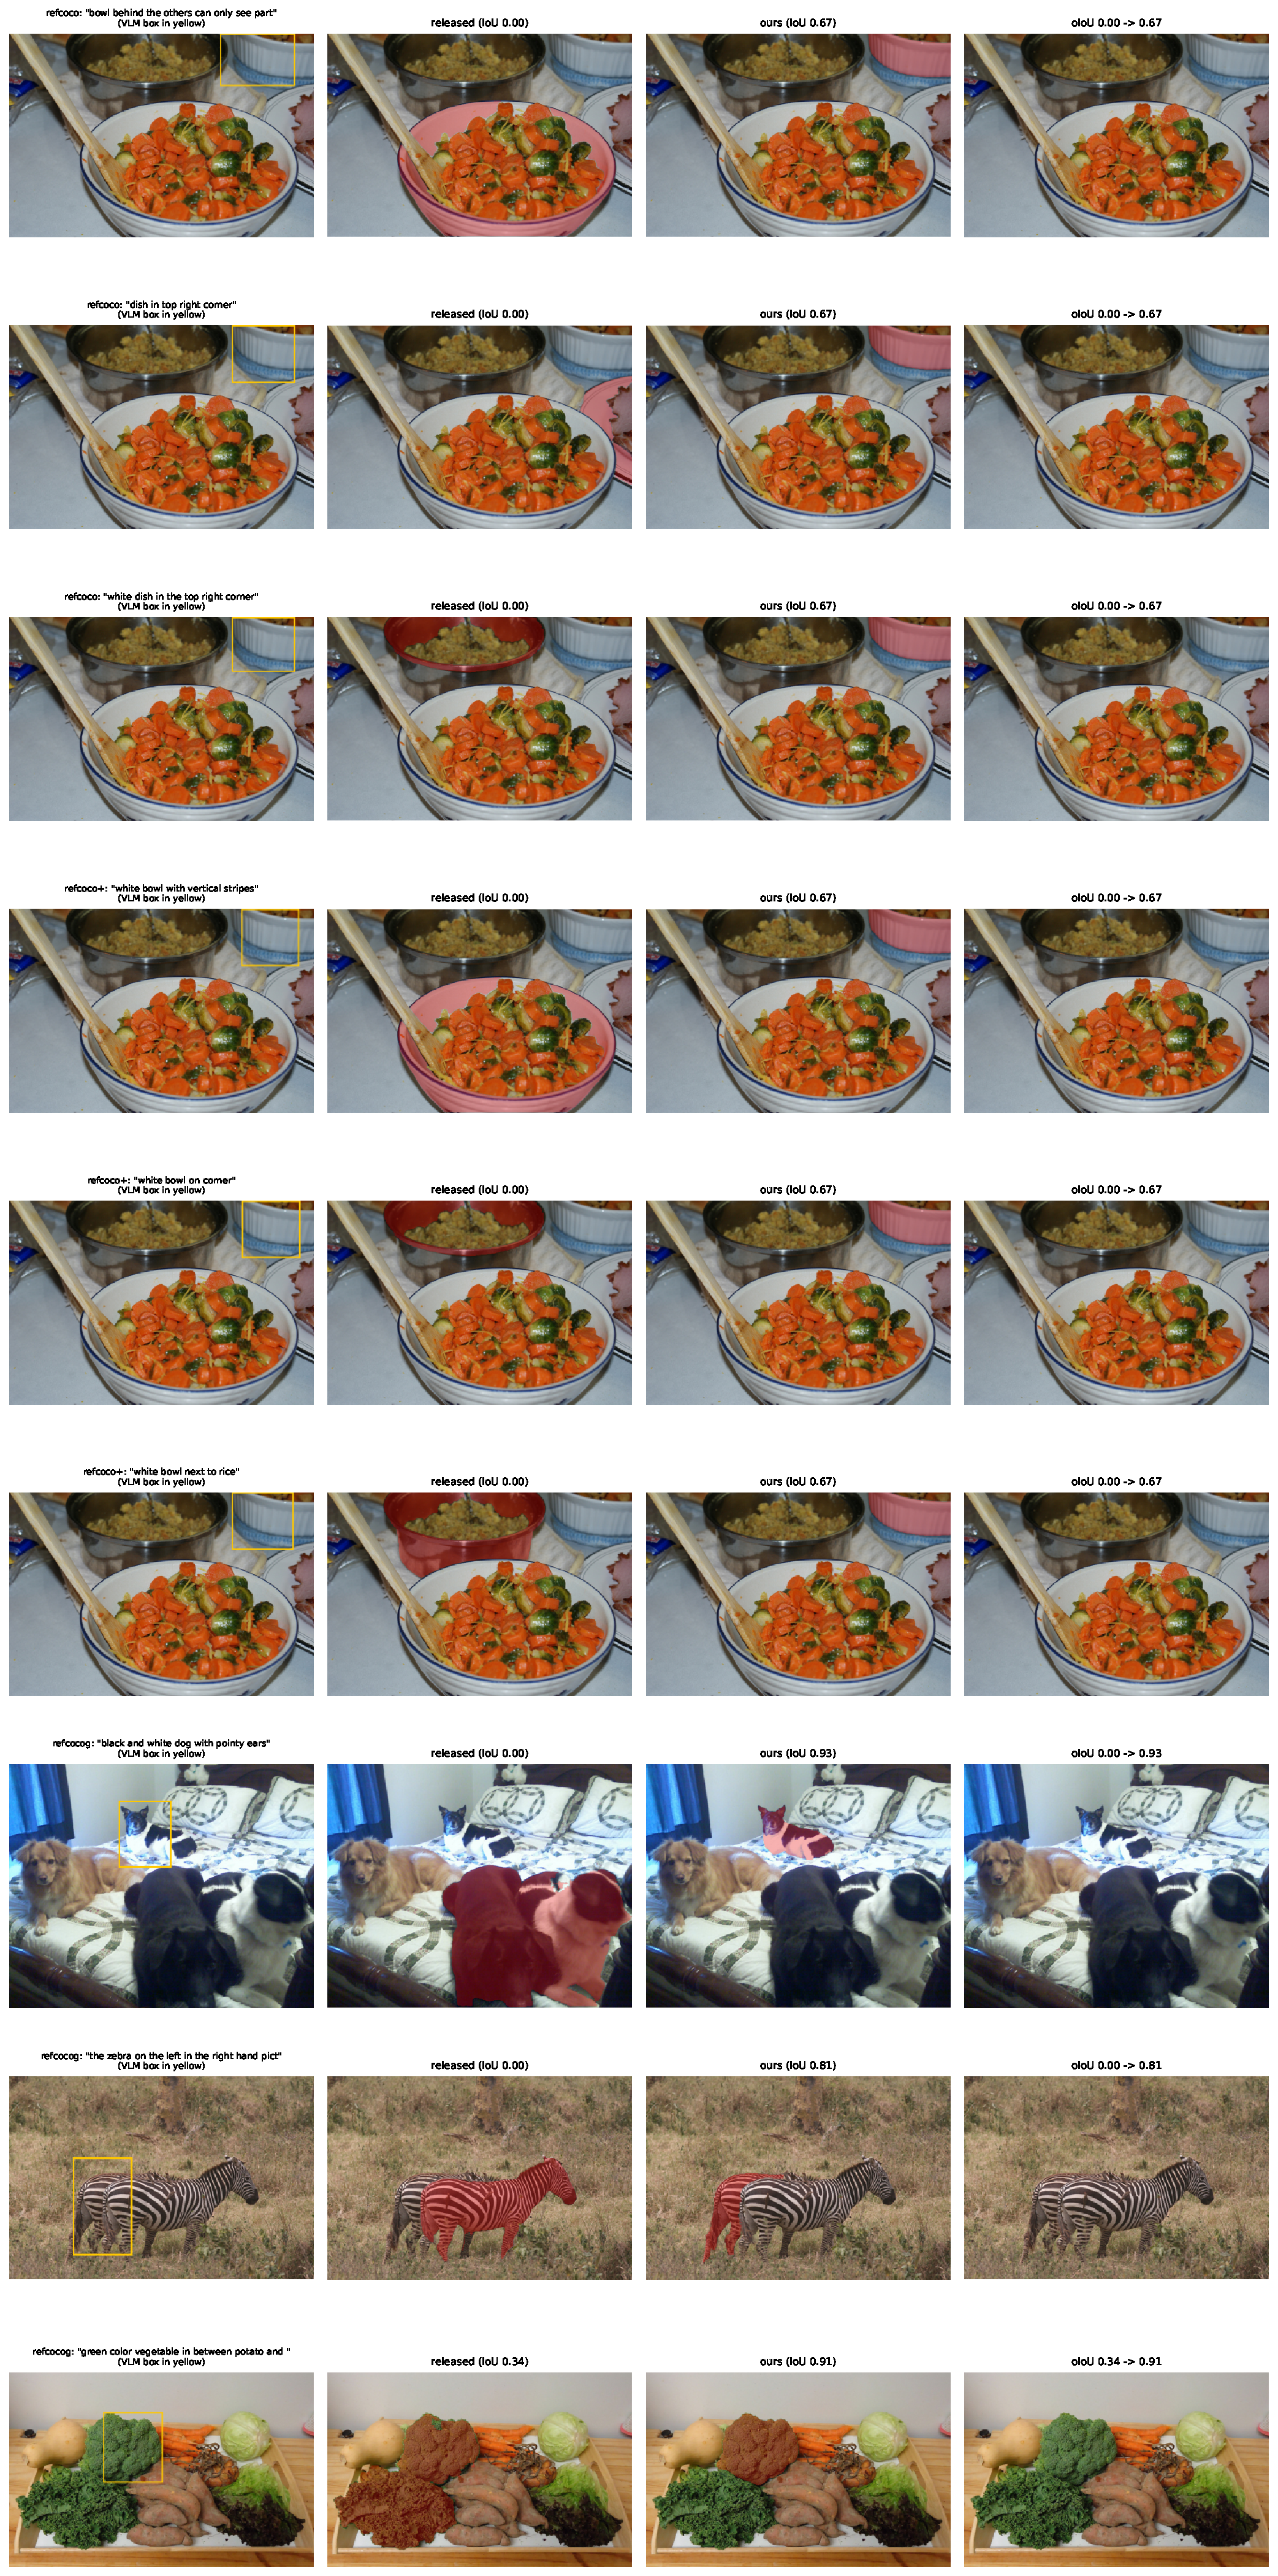
\includegraphics[height=0.90\textheight,keepaspectratio]{figures/qualitative.pdf}%
}{%
  \fbox{\parbox{0.9\textwidth}{\centering qualitative panel pending (exp/exp45\_qualitative.py)}}%
}
\caption{Examples where the box prior changes the selection (one per dataset
family, selected by a criterion fixed in \texttt{exp/exp45\_qualitative.py}:
the method and the released pipeline disagree and the IoU gap exceeds $0.25$).
Column 1 shows the VLM box (yellow) overlaid on the image and the expression;
columns 2--3 the released selection and ours. Ground-truth IoU is in each
title. These are illustrative, not a random sample.}
\label{fig:qual}
\end{figure*}

\section{Appendix: evidence map}
\label{app:evidence}

Every claim in the paper maps to a stored artifact:
\texttt{exp/out\_final/main\_\{refcoco,refcocoplus,refcocog,grefcoco\}.json}
(one per dataset; all rows, CIs, strata, quartiles, taxonomy);
\texttt{exp/out\_final/gref\_topk\_reselection.json} and
\texttt{gref\_learned\_selector\_transfer.json} (change 16 and the documented
negative transfer result);
\texttt{exp/out\_final/protocol\_audit.json} (the metric-protocol audit of
\S\ref{sec:protocol}: per-dataset protocol source, metric definition, and the
re-evaluation of the saved predictions under it, with the numbers after
alignment --- including the completed gRefCOCO coverage and the pooled oIoU);
\texttt{exp/out\_final/ablation.json} (each row with its own evidence file);
\texttt{exp/out\_final/sota\_table.json} (measured rows carry evidence paths;
published rows carry transcription sources);
\texttt{refine-logs/METHOD\_GRAVEYARD.md} (killed methods and the control
that killed each);
\texttt{paper/figures/specs/architecture.json} and the rendered
\texttt{architecture.pdf} (deterministic vector figure);
\texttt{exp/out\_extreme/records\_*.jsonl} (the scoring passes every analysis
reads);
\texttt{exp/out\_final/headroom.json} (the structural cause: top-3
containment, oracle rank, category-score top-8);
\texttt{exp/out\_final/cross\_dataset.json} (the dose-response and the
residual strata);
\texttt{exp/out\_final/pool\_robustness.json} (points-per-side 8 vs 16);
\texttt{exp/out\_final/evidence/repro\_blocks.json} with the raw logs
\texttt{repro\_official\_blockA.log} and \texttt{repro\_official\_blockB.log}
(the two disjoint reproduction-audit blocks);
\texttt{exp/out\_final/optuna\_study\_\{noun,sent\}.json} (the two
\studyTrials{}-trial studies and their per-dataset held-out mIoU);
\texttt{exp/tuning/*\_refs.json} (the held-out split: seeded train refs);
\texttt{exp/out\_vlm\_boxes/} (one cached VLM box per expression);
\texttt{exp/out\_final/gref\_ceiling.json} (the gRefCOCO no-target wall:
oracle set-IoU, the leaky logistic bound, and the $\mathrm{N\text{-}acc}$
requirement at perfect masks);
\texttt{exp/out\_final/exp37\_\{refcoco,refcocog\}\_gt.json} and
\texttt{exp37\_vlm\_sample800.json} (the box-prior ceiling and its
realistic-box sample);
\texttt{exp/out\_final/optuna\_study\_gref\{2,3,4,5\}.json} (the gRefCOCO
held-out studies: hand rules, learned selector, decision rules, clause
features; \studyTrials{} trials each);
\texttt{exp/out\_final/gref\_exists\_probe\_sh*.json} and the
\texttt{exists} cache namespace (the single yes/no presence probe);
\texttt{exp/out\_final/gref\_ensemble\_\{roc,val\}.json},
\texttt{gref\_rule\_showdown.json}, and
\texttt{gref\_ensemble\_aggregates.json} (the three-prompt presence ensemble:
held-out rule selection, full-val frontier, and the exact union-mass
requirements behind the shipped row);
\texttt{exp/out\_final/gref\_wall.json} (the three-axis wall analysis and the
exact oracle-realization requirement);
\texttt{exp/out\_final/gref\_tuned\_val2000.json} and
\texttt{exp/out\_final/gref\_full\_val.json} (the frozen gRefCOCO model's
validation evaluation).


{\small
\bibliographystyle{ieeenat_fullname}
\bibliography{references}
}

\end{document}
